\chapter{Análise dos Resultados}
\label{cap:resultados}

Este capítulo reúne os resultados do banco consolidado, segundo os métodos do Capítulo \ref{cap:matmet}. A análise descritiva cobre perfil epidemiológico, dinâmica temporal, distribuição espacial da incidência e caracterização socioespacial e climática nos níveis nacional e de Grandes Regiões, além da estratificação dos municípios, da autocorrelação espacial e da varredura espacial.

\section{Análise Descritiva}
\label{sec:descritiva}

\subsection{Perfil epidemiológico dos casos prováveis}

No perfil epidemiológico bruto, entre 2010 e 2025 foram contabilizados \TotalCasosProvaveis{} registros não descartados de dengue. O painel espacial harmonizado à malha municipal de 2010 reúne \ScanTotalCasos{} casos em \NumMunicipios{} municípios. A diferença entre os totais decorre dos critérios de classificação e inclusão territorial descritos em Métodos. No período, foram registrados \TotalObitos{} óbitos pela doença, o que corresponde a uma letalidade de \Letalidade{} no universo descritivo. A taxa de incidência acumulada nacional do painel espacial, calculada com a população média municipal do período, foi de \TIAccumBrasil{} casos por 100 mil habitantes.

O perfil demográfico dos casos é apresentado na Tabela~\ref{tab:perfil_demografico}. As mulheres corresponderam a \PctSexoFeminino{} dos casos, enquanto os homens representaram \PctSexoMasculino{}. Quanto à faixa etária, a maior concentração de casos ocorreu entre adultos jovens, com \PctFaixaVinteATrintaNove{} dos casos no grupo de 20 a 39 anos, seguida do grupo de 40 a 59 anos; a população de 60 anos ou mais respondeu por \PctFaixaSessentaMais{} dos casos e crianças de 0 a 4 anos por \PctFaixaZeroAQuatro{}.

\begin{table}[H]
\centering
\caption{Perfil demográfico dos casos prováveis de dengue, Brasil, 2010--2025.}
\label{tab:perfil_demografico}
\centering\begingroup\fontsize{9}{11}\selectfont

\resizebox{\ifdim\width>\linewidth\linewidth\else\width\fi}{!}{
\begin{tabular}{lc}
\toprule
Indicador & Valor\\
\midrule
Total de casos prováveis & 22.187.924\\
\addlinespace[0.3em]
\multicolumn{2}{l}{\textbf{Sexo (\%)}}\\
\hspace{1em}Feminino & 54,9\\
\hspace{1em}Masculino & 44,9\\
\hspace{1em}Ignorado & 0,1\\
\addlinespace[0.3em]
\multicolumn{2}{l}{\textbf{Faixa etária (\%)}}\\
\hspace{1em}0 a 4 & 2,6\\
\hspace{1em}5 a 9 & 5,2\\
\hspace{1em}10 a 14 & 7,3\\
\hspace{1em}15 a 19 & 9,1\\
\hspace{1em}20 a 39 & 36,8\\
\hspace{1em}40 a 59 & 25,9\\
\hspace{1em}60 ou mais & 11,9\\
\hspace{1em}Ignorado & 1,2\\
\addlinespace[0.3em]
\multicolumn{2}{l}{\textbf{Desfecho}}\\
\hspace{1em}Óbitos & 16.975\\
\hspace{1em}Letalidade (\%) & 0,08\\
\bottomrule
\end{tabular}}
\endgroup{}

\par\vspace{0.4em}
\parbox{0.9\linewidth}{\footnotesize\textit{Nota:} Percentuais calculados sobre os casos prováveis com informação válida ou categoria de ignorado explicitamente reportada.}
\end{table}

\subsection{Série temporal e sazonalidade}

A Figura~\ref{fig:serie_temporal} apresenta, no painel (a), a evolução anual da taxa de incidência nacional e, no painel (b), o padrão sazonal médio mensal de casos prováveis. A série alterna picos e anos de menor transmissão. O ano de 2024 teve o maior volume no período 2010--2025, com \CasosDoisMilVinteQuatro{} casos prováveis e incidência de \TIDoisMilVinteQuatro{} casos por 100 mil habitantes. No painel espacial, 2025 reuniu \CasosDoisMilVinteCinco{} casos e foi o terceiro ano mais intenso no período 2010--2025, atrás de 2024 e 2015. Os anos de 2020 e 2021 coincidem com o período de reorganização da vigilância durante a pandemia de Covid-19.

\begin{figure}[H]
    \centering
    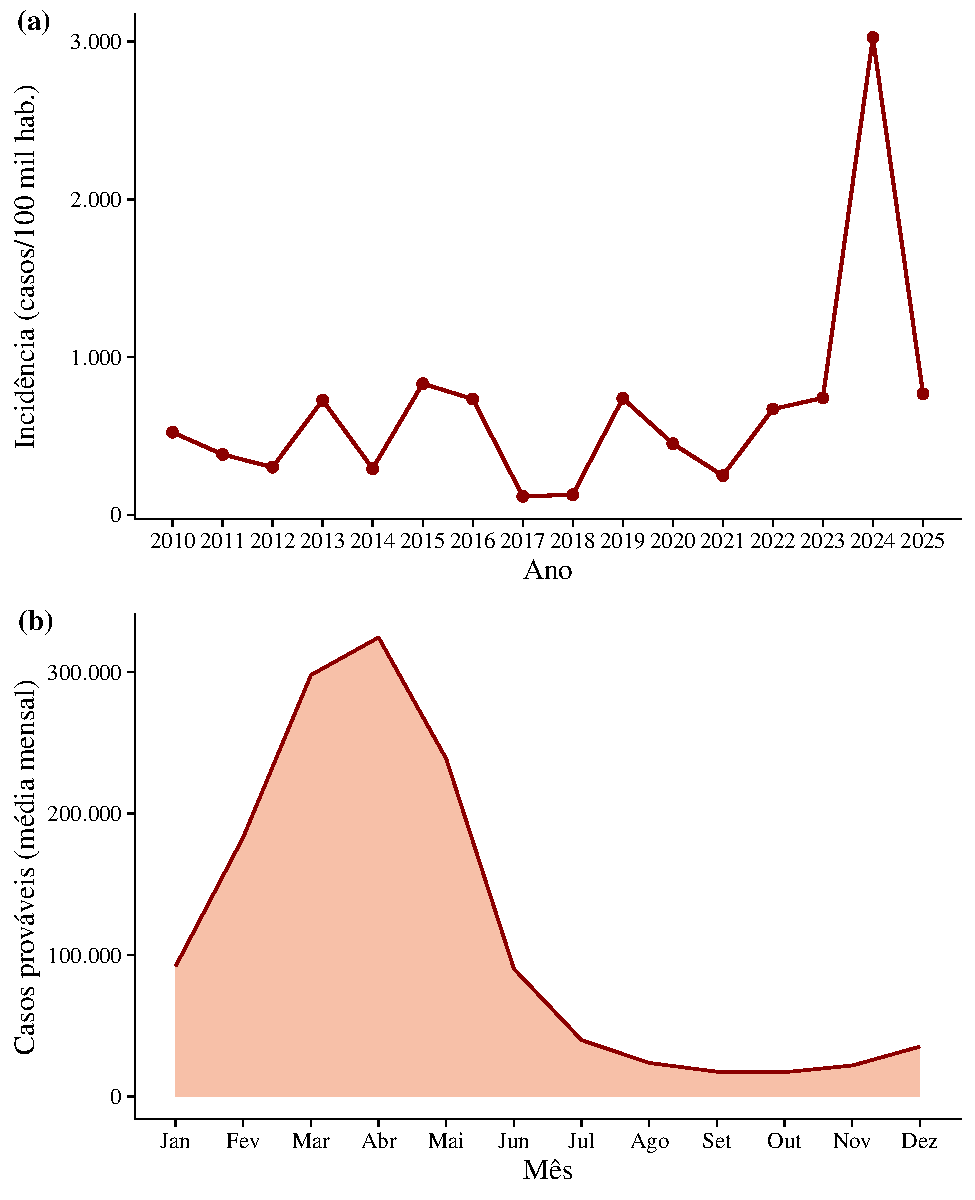
\includegraphics[width=0.95\textwidth]{fig_serie_temporal_dengue.pdf}
    \caption{Série temporal da dengue no Brasil, 2010--2025: (a) taxa de incidência anual, em casos prováveis por 100 mil habitantes; (b) média mensal de casos prováveis, em casos. Fontes: SINAN e IBGE.}
    \label{fig:serie_temporal}
\end{figure}

O padrão sazonal observado no painel (b) concentra a transmissão no primeiro semestre, com máximo em abril, seguido de março e de maio.

\subsection{Distribuição regional da incidência}

A Figura~\ref{fig:series_regioes} apresenta as séries temporais anuais da incidência por Grande Região, com a linha tracejada representando o valor nacional como referência. As regiões Centro-Oeste e Sudeste concentraram as maiores incidências acumuladas do período, com taxas de \TIRegiaoCentroOeste{} e \TIRegiaoSudeste{} casos por 100 mil habitantes, respectivamente, seguidas pelas regiões Sul (\TIRegiaoSul{}), Nordeste (\TIRegiaoNordeste{}) e Norte (\TIRegiaoNorte{}).

\begin{figure}[H]
    \centering
    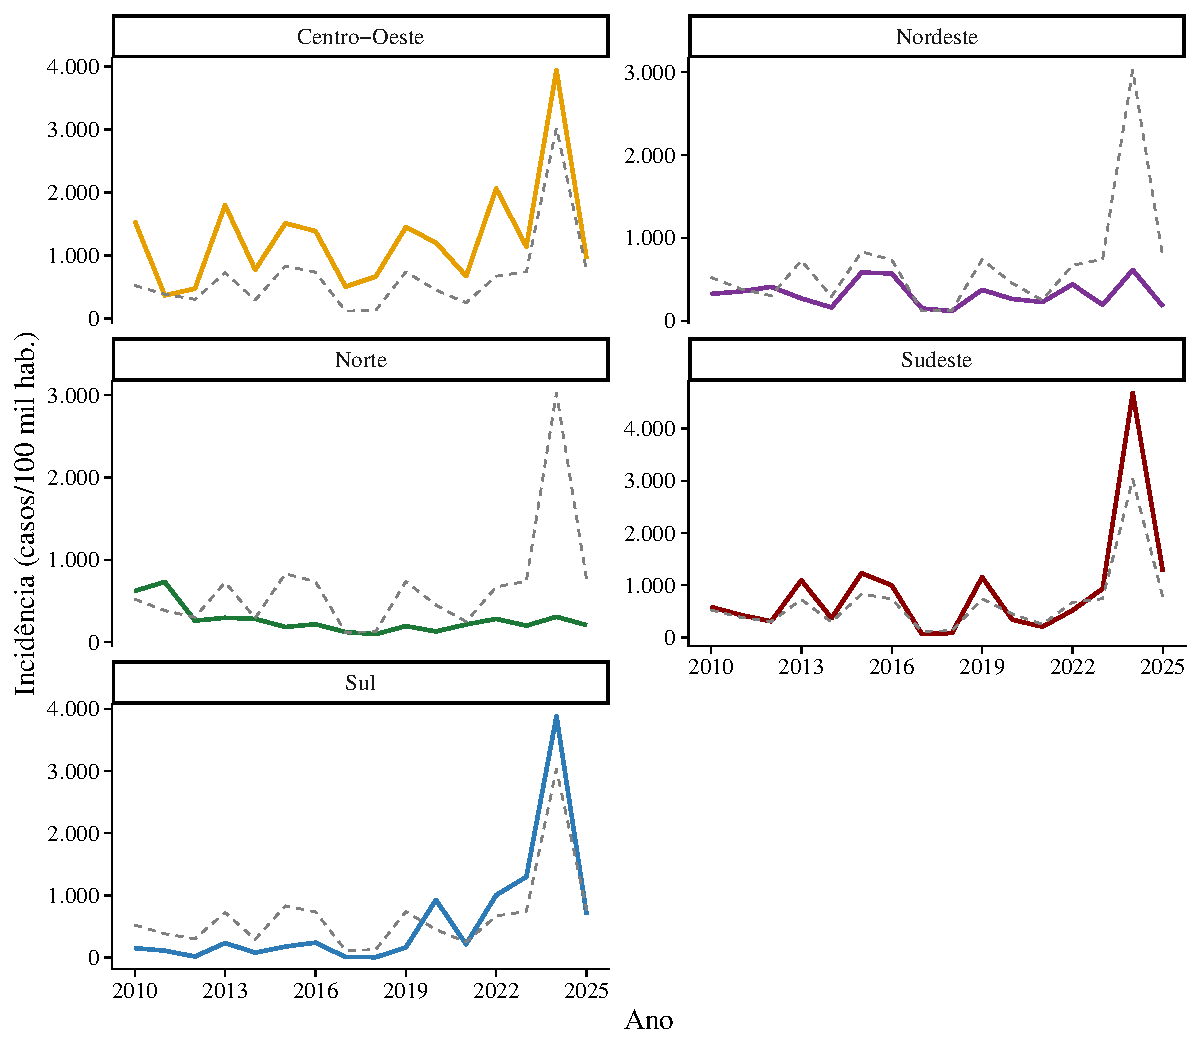
\includegraphics[width=0.95\textwidth]{fig_series_regioes.pdf}
    \caption{Taxa de incidência anual de dengue por Grande Região, Brasil, 2010--2025, em casos por 100 mil habitantes, com referência nacional tracejada. Fontes: SINAN e IBGE.}
    \label{fig:series_regioes}
\end{figure}

\begin{figure}[H]
    \centering
    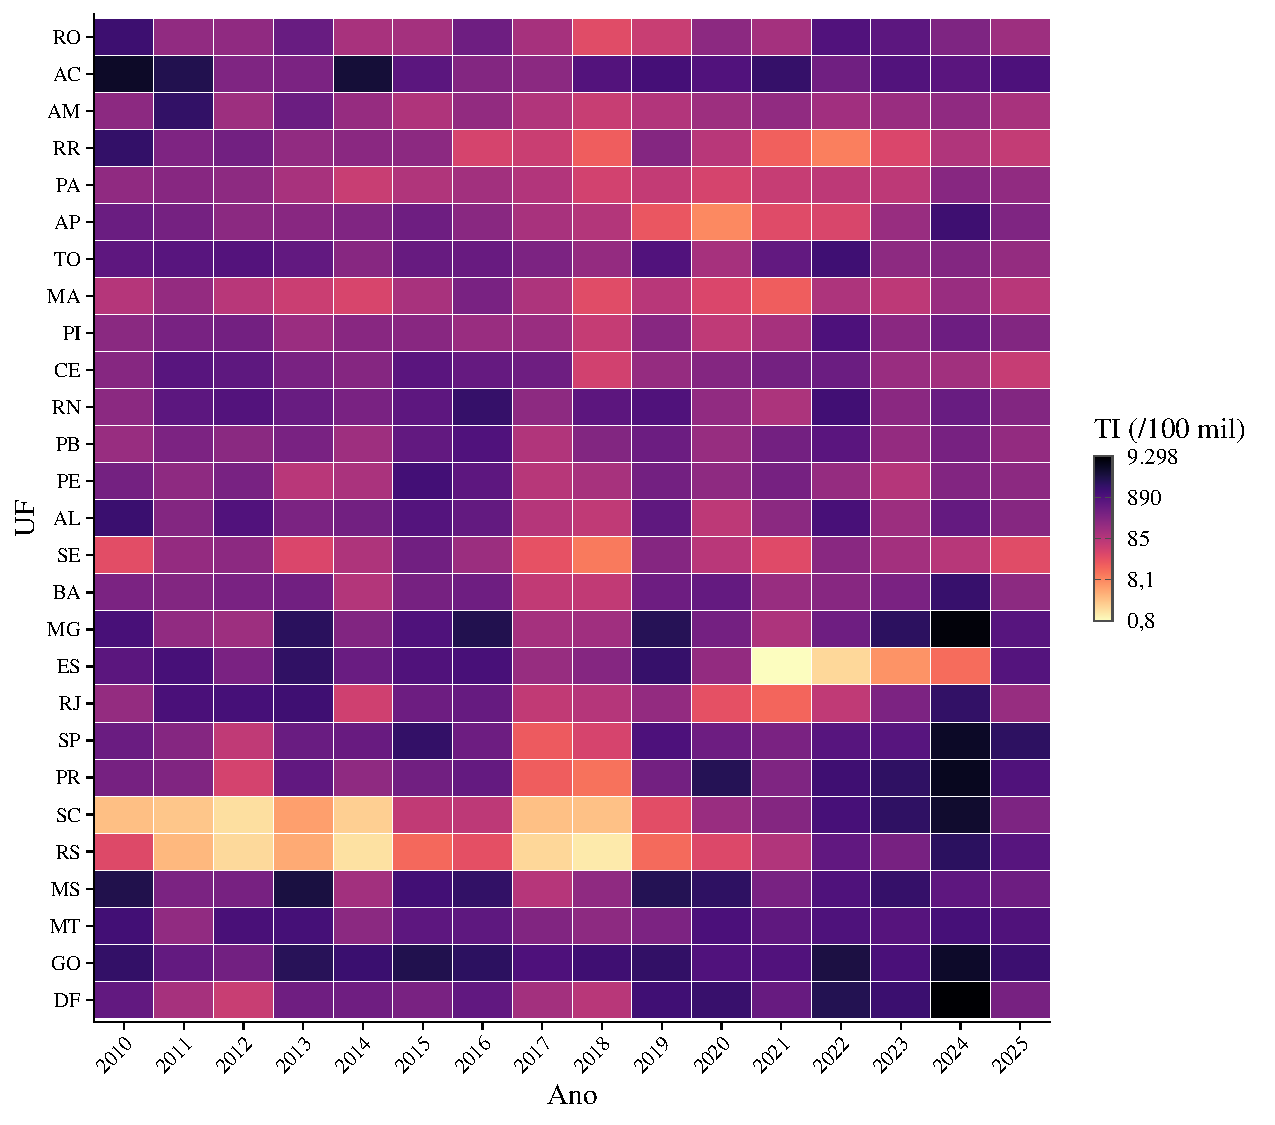
\includegraphics[width=0.95\textwidth]{fig_heatmap_incidencia_uf_ano.pdf}
    \caption{Taxa de incidência de dengue por UF e ano, Brasil, 2010--2025, em casos por 100 mil habitantes, com cor em logaritmo de base 10. Fontes: SINAN e IBGE.}
    \label{fig:heatmap_uf_ano}
    \vspace{0.3em}
    {\footnotesize\noindent\textit{Nota:} A taxa vai de \TIMinTI{} (\TIMinUF{} em \TIMinUFAno{}) a \TIMaxTI{} (\TIMaxUF{} em \TIMaxUFAno{}); em escala linear, os valores baixos comprimem a escala e reduzem o contraste.\par}
\end{figure}

A Figura~\ref{fig:heatmap_uf_ano} abre o mesmo dado por UF e ano. O ano de 2024 corresponde ao máximo de incidência em 10 das 27 UFs; em seguida vêm 2010, com 5 UFs, e 2011 e 2016, com 3 cada. Na Região Sul, as incidências anuais elevaram-se a partir da segunda metade do período 2010--2025.

\subsection{Autocorrelação espacial}

A Figura~\ref{fig:evolucao_moran} apresenta a evolução anual do Índice Global de Moran para a taxa de incidência municipal, calculado com matriz de vizinhança por contiguidade. O índice foi positivo e estatisticamente significativo em todos os anos do período (nível de 5\%), variando de \MoranMin{} a \MoranMax{}.

\begin{figure}[H]
    \centering
    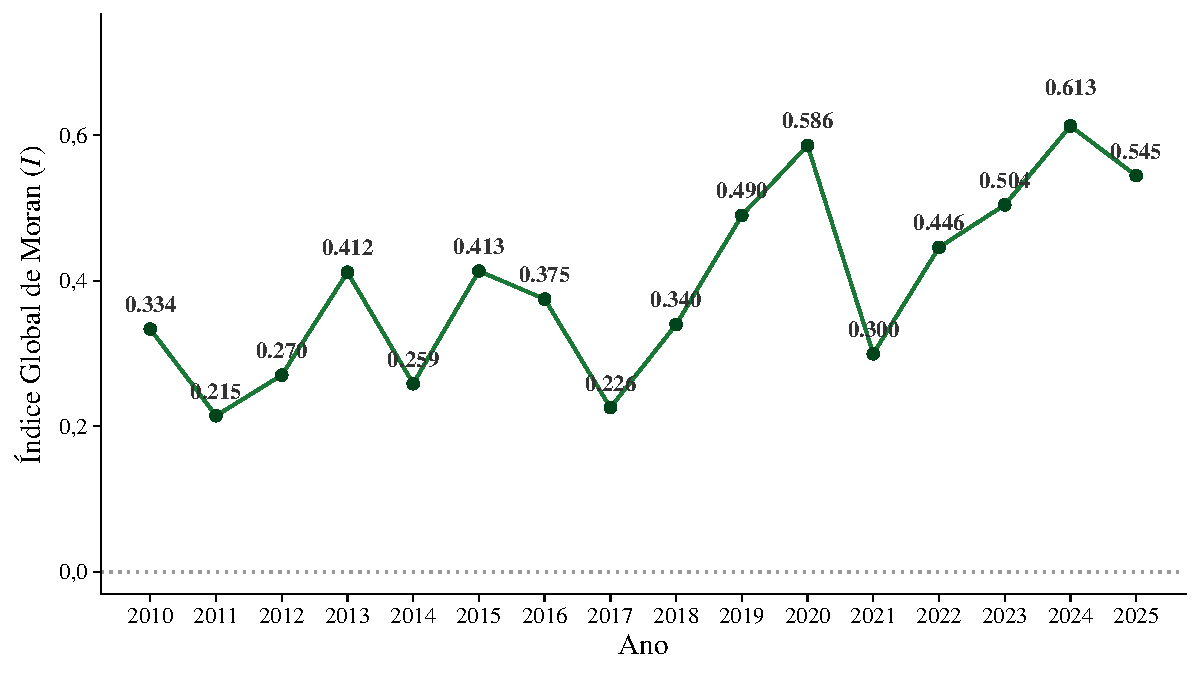
\includegraphics[width=0.95\textwidth]{fig_evolucao_moran.pdf}
    \caption{Evolução anual do Índice Global de Moran para a taxa de incidência municipal de dengue, Brasil, 2010--2025, calculado sobre casos prováveis por 100 mil habitantes. Fontes: SINAN e IBGE.}
    \label{fig:evolucao_moran}
\end{figure}

A autocorrelação espacial variou ao longo do tempo, com valores mais elevados nos anos de 2020 e, em especial, 2024 (\MoranDoisMilVinteQuatro{}), onde a incidência atingiu seu máximo. Valores relativamente menores foram encontrados nos anos 2011, 2017 e 2014.

Para identificar onde se concentram os \textit{clusters} de alto e de baixo risco, aplicou-se o Moran Local (LISA) à razão acumulada de casos por população média no período (2010--2025), com a mesma estrutura de vizinhança do índice global e 999 simulações condicionais (nível nominal de 5\%), sem correção para comparações múltiplas. A Figura~\ref{fig:mapa_lisa} apresenta a classificação dos municípios nos quadrantes do diagrama de dispersão de Moran: \LisaSig{} municípios (\LisaPctSig{}) foram classificados como associação local significativa pelo valor-p bilateral por simulação, dos quais \LisaHH{} (\LisaPctHH{}) formam o quadrante alto-alto e \LisaLL{} (\LisaPctLL{}) o quadrante baixo-baixo; os quadrantes alto-baixo e baixo-alto reuniram apenas \LisaHL{} e \LisaLH{} municípios, respectivamente, enquanto os \LisaNS{} municípios restantes (\LisaPctNS{}) não atingiram o nível nominal de significância.

\begin{figure}[H]
    \centering
    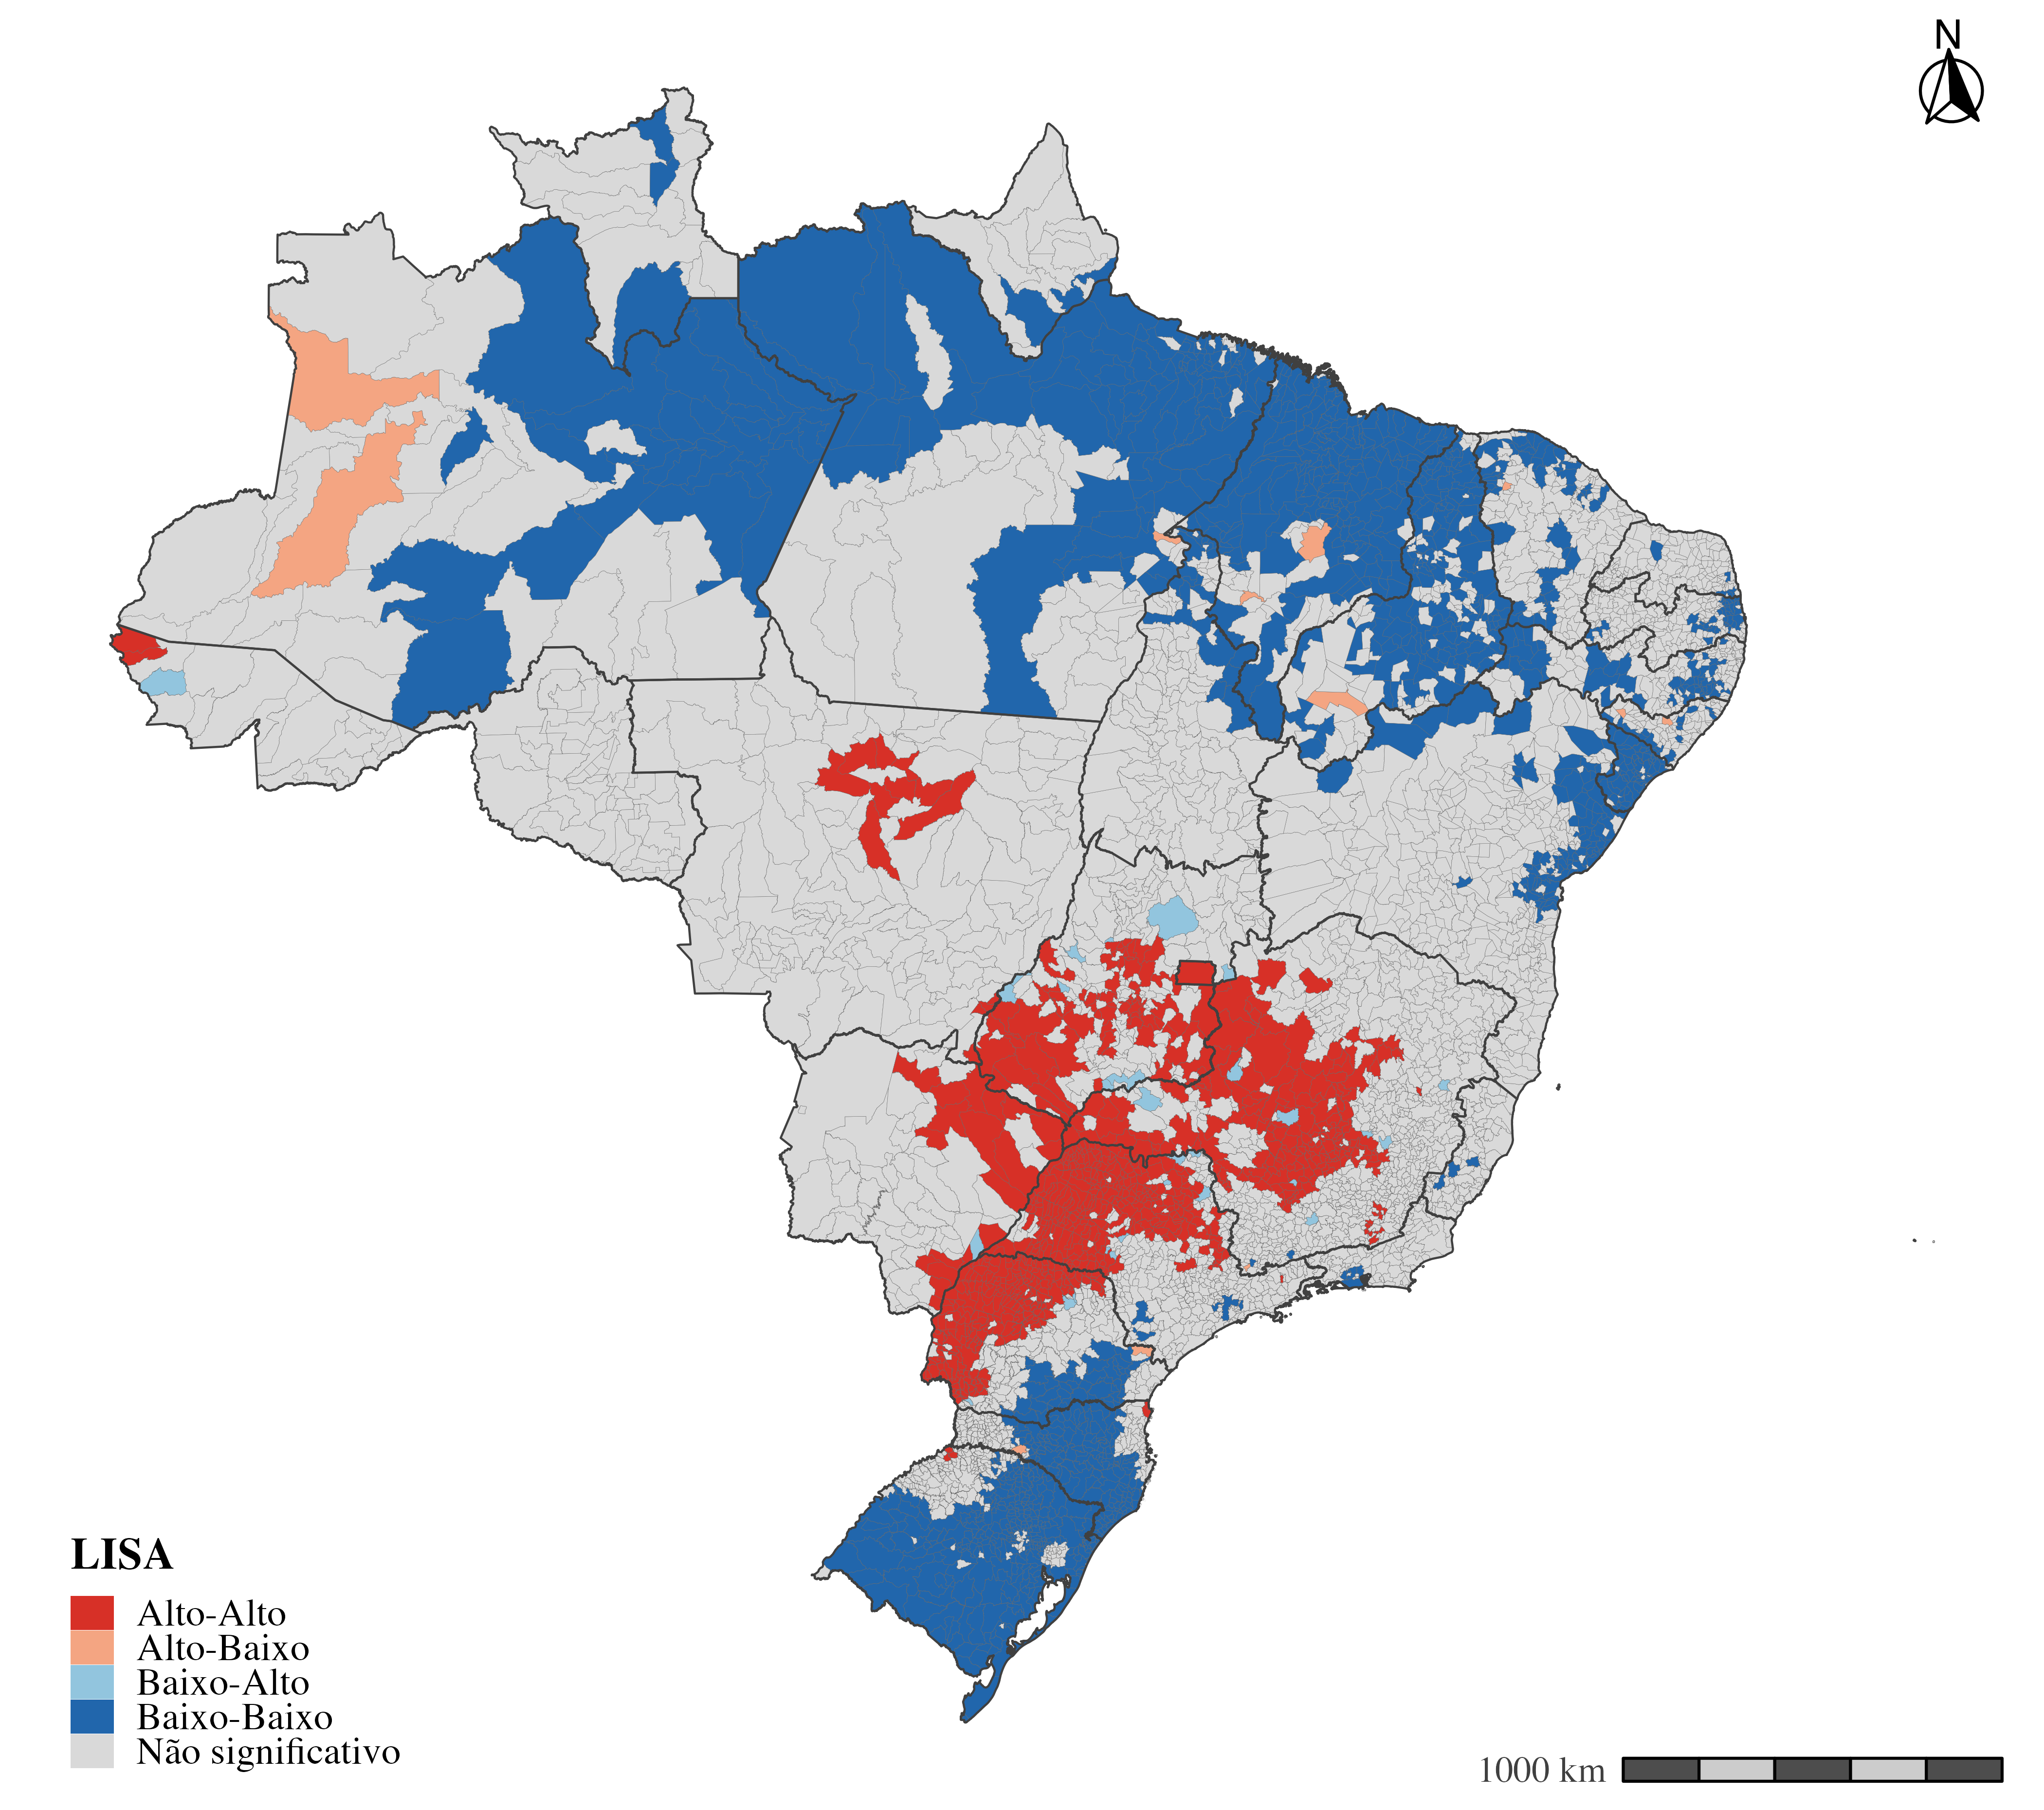
\includegraphics[width=0.64\textwidth]{fig_mapa_lisa.png}
    \caption{Quadrantes locais de associação espacial da razão acumulada de casos por população média, Brasil, 2010--2025. Fontes: SINAN e IBGE.}
    \label{fig:mapa_lisa}
    \vspace{0.3em}
    {\footnotesize\noindent\textit{Nota:} Classificação local com 999 simulações condicionais e nível nominal de 5\%.\par}
\end{figure}

\subsection{Caracterização socioespacial e climática}

As Tabelas~\ref{tab:resumo_socioespacial} e \ref{tab:resumo_clima} sintetizam, por Grande Região e para o Brasil, as medidas-resumo das variáveis socioespaciais (Censo 2022) e climáticas (reanálise climática), respectivamente.

\begin{table}[!h]
\centering
\caption{\label{tab:resumo_socioespacial}Medidas-resumo das variáveis socioespaciais por Grande Região (Censo 2022).}
\centering
\resizebox{\ifdim\width>\linewidth\linewidth\else\width\fi}{!}{
\fontsize{9}{11}\selectfont
\begin{tabular}[t]{lcccccc}
\toprule
Medida & Brasil & Norte & Nordeste & Sudeste & Sul & Centro-Oeste\\
\midrule
\addlinespace[0.3em]
\multicolumn{7}{l}{\textbf{Abastecimento de água por rede geral (\%)}}\\
\hspace{1em}Média (D.P.) & 71,7 (19,6) & 53,4 (22,8) & 67,3 (20,0) & 79,1 (15,6) & 74,3 (18,1) & 73,5 (15,4)\\
\hspace{1em}Mediana (IIQ) & 75,8 (26,2) & 57,6 (32,9) & 70,5 (25,4) & 82,8 (21,7) & 78,7 (25,8) & 75,7 (17,8)\\
\hspace{1em}Mínimo–Máximo & 0,0 – 100,0 & 0,0 – 95,0 & 0,0 – 99,6 & 22,5 – 100,0 & 10,2 – 99,6 & 3,4 – 96,6\\
\addlinespace[0.3em]
\multicolumn{7}{l}{\textbf{Esgotamento sanitário por rede (\%)}}\\
\hspace{1em}Média (D.P.) & 37,7 (33,0) & 7,4 (12,4) & 24,4 (23,9) & 70,6 (23,4) & 29,8 (29,3) & 20,7 (25,4)\\
\hspace{1em}Mediana (IIQ) & 32,3 (63,7) & 2,5 (6,4) & 17,0 (38,1) & 76,8 (32,3) & 18,9 (51,3) & 6,6 (34,0)\\
\hspace{1em}Mínimo–Máximo & 0,0 – 99,9 & 0,0 – 76,6 & 0,0 – 95,1 & 0,1 – 99,9 & 0,0 – 98,1 & 0,0 – 94,3\\
\addlinespace[0.3em]
\multicolumn{7}{l}{\textbf{Coleta de lixo (\%)}}\\
\hspace{1em}Média (D.P.) & 80,2 (17,4) & 66,2 (17,0) & 70,7 (17,8) & 89,1 (12,5) & 86,8 (13,5) & 81,6 (13,0)\\
\hspace{1em}Mediana (IIQ) & 85,1 (25,5) & 66,7 (25,8) & 72,5 (25,1) & 94,2 (12,3) & 91,3 (16,4) & 84,6 (17,1)\\
\hspace{1em}Mínimo–Máximo & 1,7 – 100,0 & 13,6 – 98,8 & 1,7 – 99,6 & 24,1 – 100,0 & 31,3 – 100,0 & 29,1 – 99,8\\
\addlinespace[0.3em]
\multicolumn{7}{l}{\textbf{População em favelas (\%)}}\\
\hspace{1em}Média (D.P.) & 1,0 (4,3) & 3,1 (8,9) & 0,8 (3,9) & 1,2 (4,2) & 0,5 (2,5) & 0,2 (1,1)\\
\hspace{1em}Mediana (IIQ) & 0,0 (0,0) & 0,0 (0,0) & 0,0 (0,0) & 0,0 (0,0) & 0,0 (0,0) & 0,0 (0,0)\\
\hspace{1em}Mínimo–Máximo & 0,0 – 69,2 & 0,0 – 69,2 & 0,0 – 45,4 & 0,0 – 42,6 & 0,0 – 47,2 & 0,0 – 11,8\\
\addlinespace[0.3em]
\multicolumn{7}{l}{\textbf{Densidade demográfica (hab/km²)}}\\
\hspace{1em}Média (D.P.) & 113,8 (585,8) & 23,1 (142,2) & 89,1 (395,6) & 205,7 (942,0) & 87,0 (285,8) & 36,1 (207,1)\\
\hspace{1em}Mediana (IIQ) & 24,1 (41,8) & 4,1 (9,0) & 28,6 (48,5) & 30,8 (53,0) & 25,5 (33,9) & 5,8 (12,2)\\
\hspace{1em}Mínimo–Máximo & 0,2 – 13.328,0 & 0,2 – 2.501,1 & 1,0 – 7.958,5 & 1,2 – 13.328,0 & 1,5 – 4.065,9 & 0,3 – 3.221,8\\
\bottomrule
\end{tabular}}
\end{table}


\begin{table}[!h]
\centering
\caption{\label{tab:resumo_clima}Medidas-resumo das variáveis climáticas por Grande Região, Brasil, 2010--2025.}
\centering
\resizebox{\ifdim\width>\linewidth\linewidth\else\width\fi}{!}{
\fontsize{9}{11}\selectfont
\begin{tabular}[t]{lcccccc}
\toprule
Medida & Brasil & Norte & Nordeste & Sudeste & Sul & Centro-Oeste\\
\midrule
\addlinespace[0.3em]
\multicolumn{7}{l}{\textbf{Temperatura máxima extrema anual (°C)}}\\
\hspace{1em}Média (D.P.) & 35,2 (2,5) & 36,2 (1,8) & 35,4 (2,4) & 34,9 (2,6) & 33,9 (2,4) & 37,4 (1,6)\\
\hspace{1em}Mediana (IIQ) & 35,4 (3,8) & 36,4 (2,3) & 35,8 (3,7) & 35,0 (3,6) & 34,0 (3,5) & 37,4 (2,2)\\
\hspace{1em}Mínimo–Máximo & 25,6 – 42,7 & 30,0 – 40,9 & 28,6 – 40,6 & 25,6 – 42,7 & 25,8 – 41,2 & 32,2 – 42,3\\
\addlinespace[0.3em]
\multicolumn{7}{l}{\textbf{Dias sob onda de calor (dias/ano)}}\\
\hspace{1em}Média (D.P.) & 24,1 (16,3) & 27,2 (21,3) & 22,7 (15,7) & 24,1 (16,7) & 22,8 (14,0) & 29,8 (15,5)\\
\hspace{1em}Mediana (IIQ) & 22,0 (22,0) & 24,0 (26,0) & 21,0 (21,0) & 22,0 (22,0) & 21,0 (21,0) & 29,0 (22,0)\\
\hspace{1em}Mínimo–Máximo & 0,0 – 151,0 & 0,0 – 151,0 & 0,0 – 100,0 & 0,0 – 104,0 & 0,0 – 83,0 & 0,0 – 86,0\\
\addlinespace[0.3em]
\multicolumn{7}{l}{\textbf{Umidade relativa média (\%)}}\\
\hspace{1em}Média (D.P.) & 70,7 (7,8) & 75,2 (8,2) & 69,3 (8,7) & 69,3 (6,6) & 75,5 (5,0) & 64,3 (5,0)\\
\hspace{1em}Mediana (IIQ) & 71,7 (12,1) & 77,5 (12,9) & 71,0 (14,9) & 69,4 (9,5) & 75,6 (6,3) & 62,9 (6,9)\\
\hspace{1em}Mínimo–Máximo & 46,3 – 90,6 & 53,3 – 90,6 & 46,3 – 86,1 & 46,8 – 87,4 & 59,0 – 87,1 & 53,3 – 83,0\\
\addlinespace[0.3em]
\multicolumn{7}{l}{\textbf{Precipitação anual acumulada (mm)}}\\
\hspace{1em}Média (D.P.) & 1.262,1 (572,7) & 1.916,6 (623,3) & 881,4 (491,3) & 1.162,2 (373,6) & 1.682,9 (438,9) & 1.380,3 (388,4)\\
\hspace{1em}Mediana (IIQ) & 1.236,3 (742,4) & 1.833,6 (808,9) & 777,5 (640,4) & 1.158,1 (470,6) & 1.650,0 (579,5) & 1.344,8 (441,8)\\
\hspace{1em}Mínimo–Máximo & 0,2 – 7.139,7 & 15,0 – 5.472,4 & 0,2 – 5.411,0 & 0,2 – 6.775,8 & 17,8 – 4.886,0 & 90,8 – 7.139,7\\
\bottomrule
\end{tabular}}
\end{table}


Em nível nacional, a cobertura média municipal de abastecimento de água por rede geral foi de \MediaMunAgua{} (atingindo \PropAguaRedeBrasil{} quando ponderada pelo número de domicílios do município), de esgotamento sanitário por rede de \MediaMunEsgoto{} (\PropEsgotoRedeBrasil{} ponderada) e de coleta de resíduos sólidos de \MediaMunLixo{} (\PropLixoBrasil{} ponderada), enquanto a proporção média de população residente em favelas e comunidades urbanas nos municípios foi de \MediaMunFavela{} (\PropFavelaBrasil{} no agregado populacional nacional). A Região Norte apresentou os menores patamares de infraestrutura de saneamento, enquanto o Sudeste concentrou os maiores indicadores de cobertura, como detalhado na Tabela~\ref{tab:resumo_socioespacial}.

Quanto ao clima, a temperatura máxima extrema anual média municipal foi de 35,2~$^\circ$C (34,6~$^\circ$C quando ponderada pela população), com umidade relativa de 70,7\% (73,6\% ponderada) e precipitação anual de 1.262,1 mm (\PrecipAnualBrasil{} ponderada). As Figuras~\ref{fig:mapa_temperatura}, \ref{fig:mapa_precipitacao} e \ref{fig:mapa_umidade} mostram a heterogeneidade climática do território: as maiores temperaturas ocorreram no Centro-Oeste; as maiores médias municipais de umidade relativa, no Sul e no Norte; a maior pluviosidade, na Amazônia e no Sul; e a menor umidade relativa, no interior do Nordeste e do Centro-Oeste. O Sul apresentou as temperaturas mais amenas.

\begin{figure}[H]
    \centering
    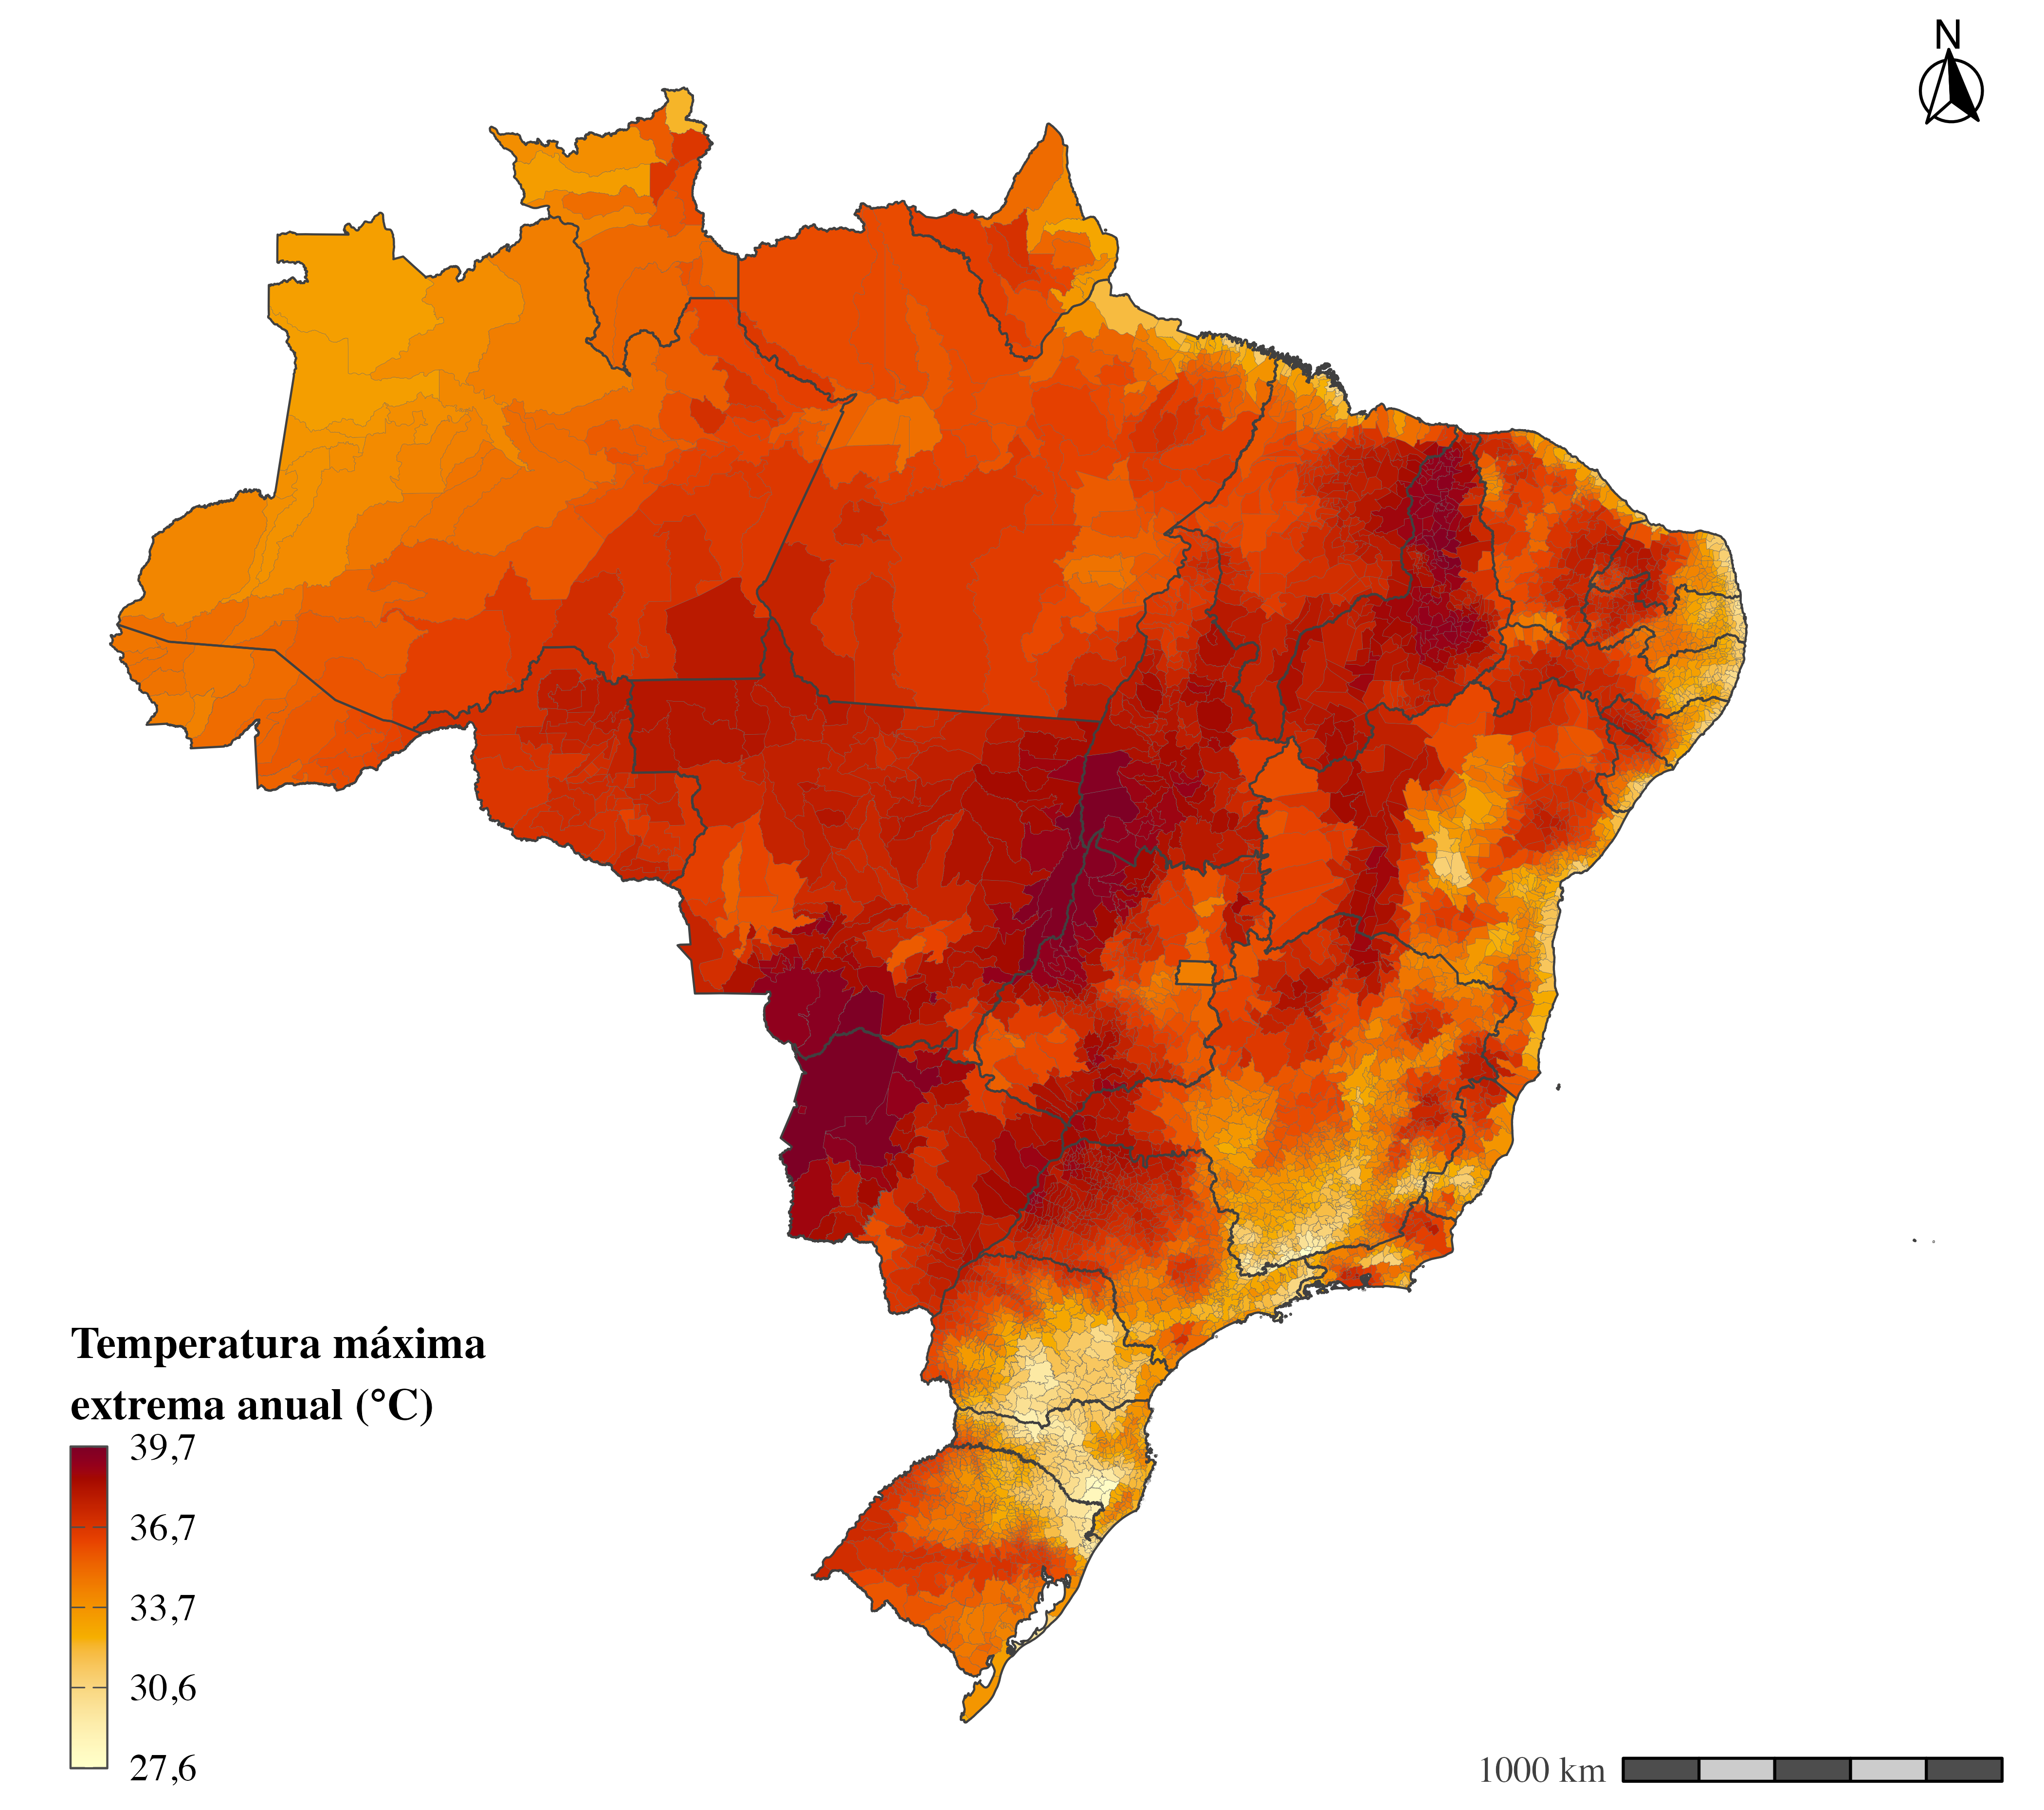
\includegraphics[width=0.64\textwidth]{fig_mapa_temperatura.png}
    \caption{Média municipal da máxima diária anual de temperatura, Brasil, 2010--2025, em graus Celsius. Fonte: reanálise climática.}
    \label{fig:mapa_temperatura}
\end{figure}

\begin{figure}[H]
    \centering
    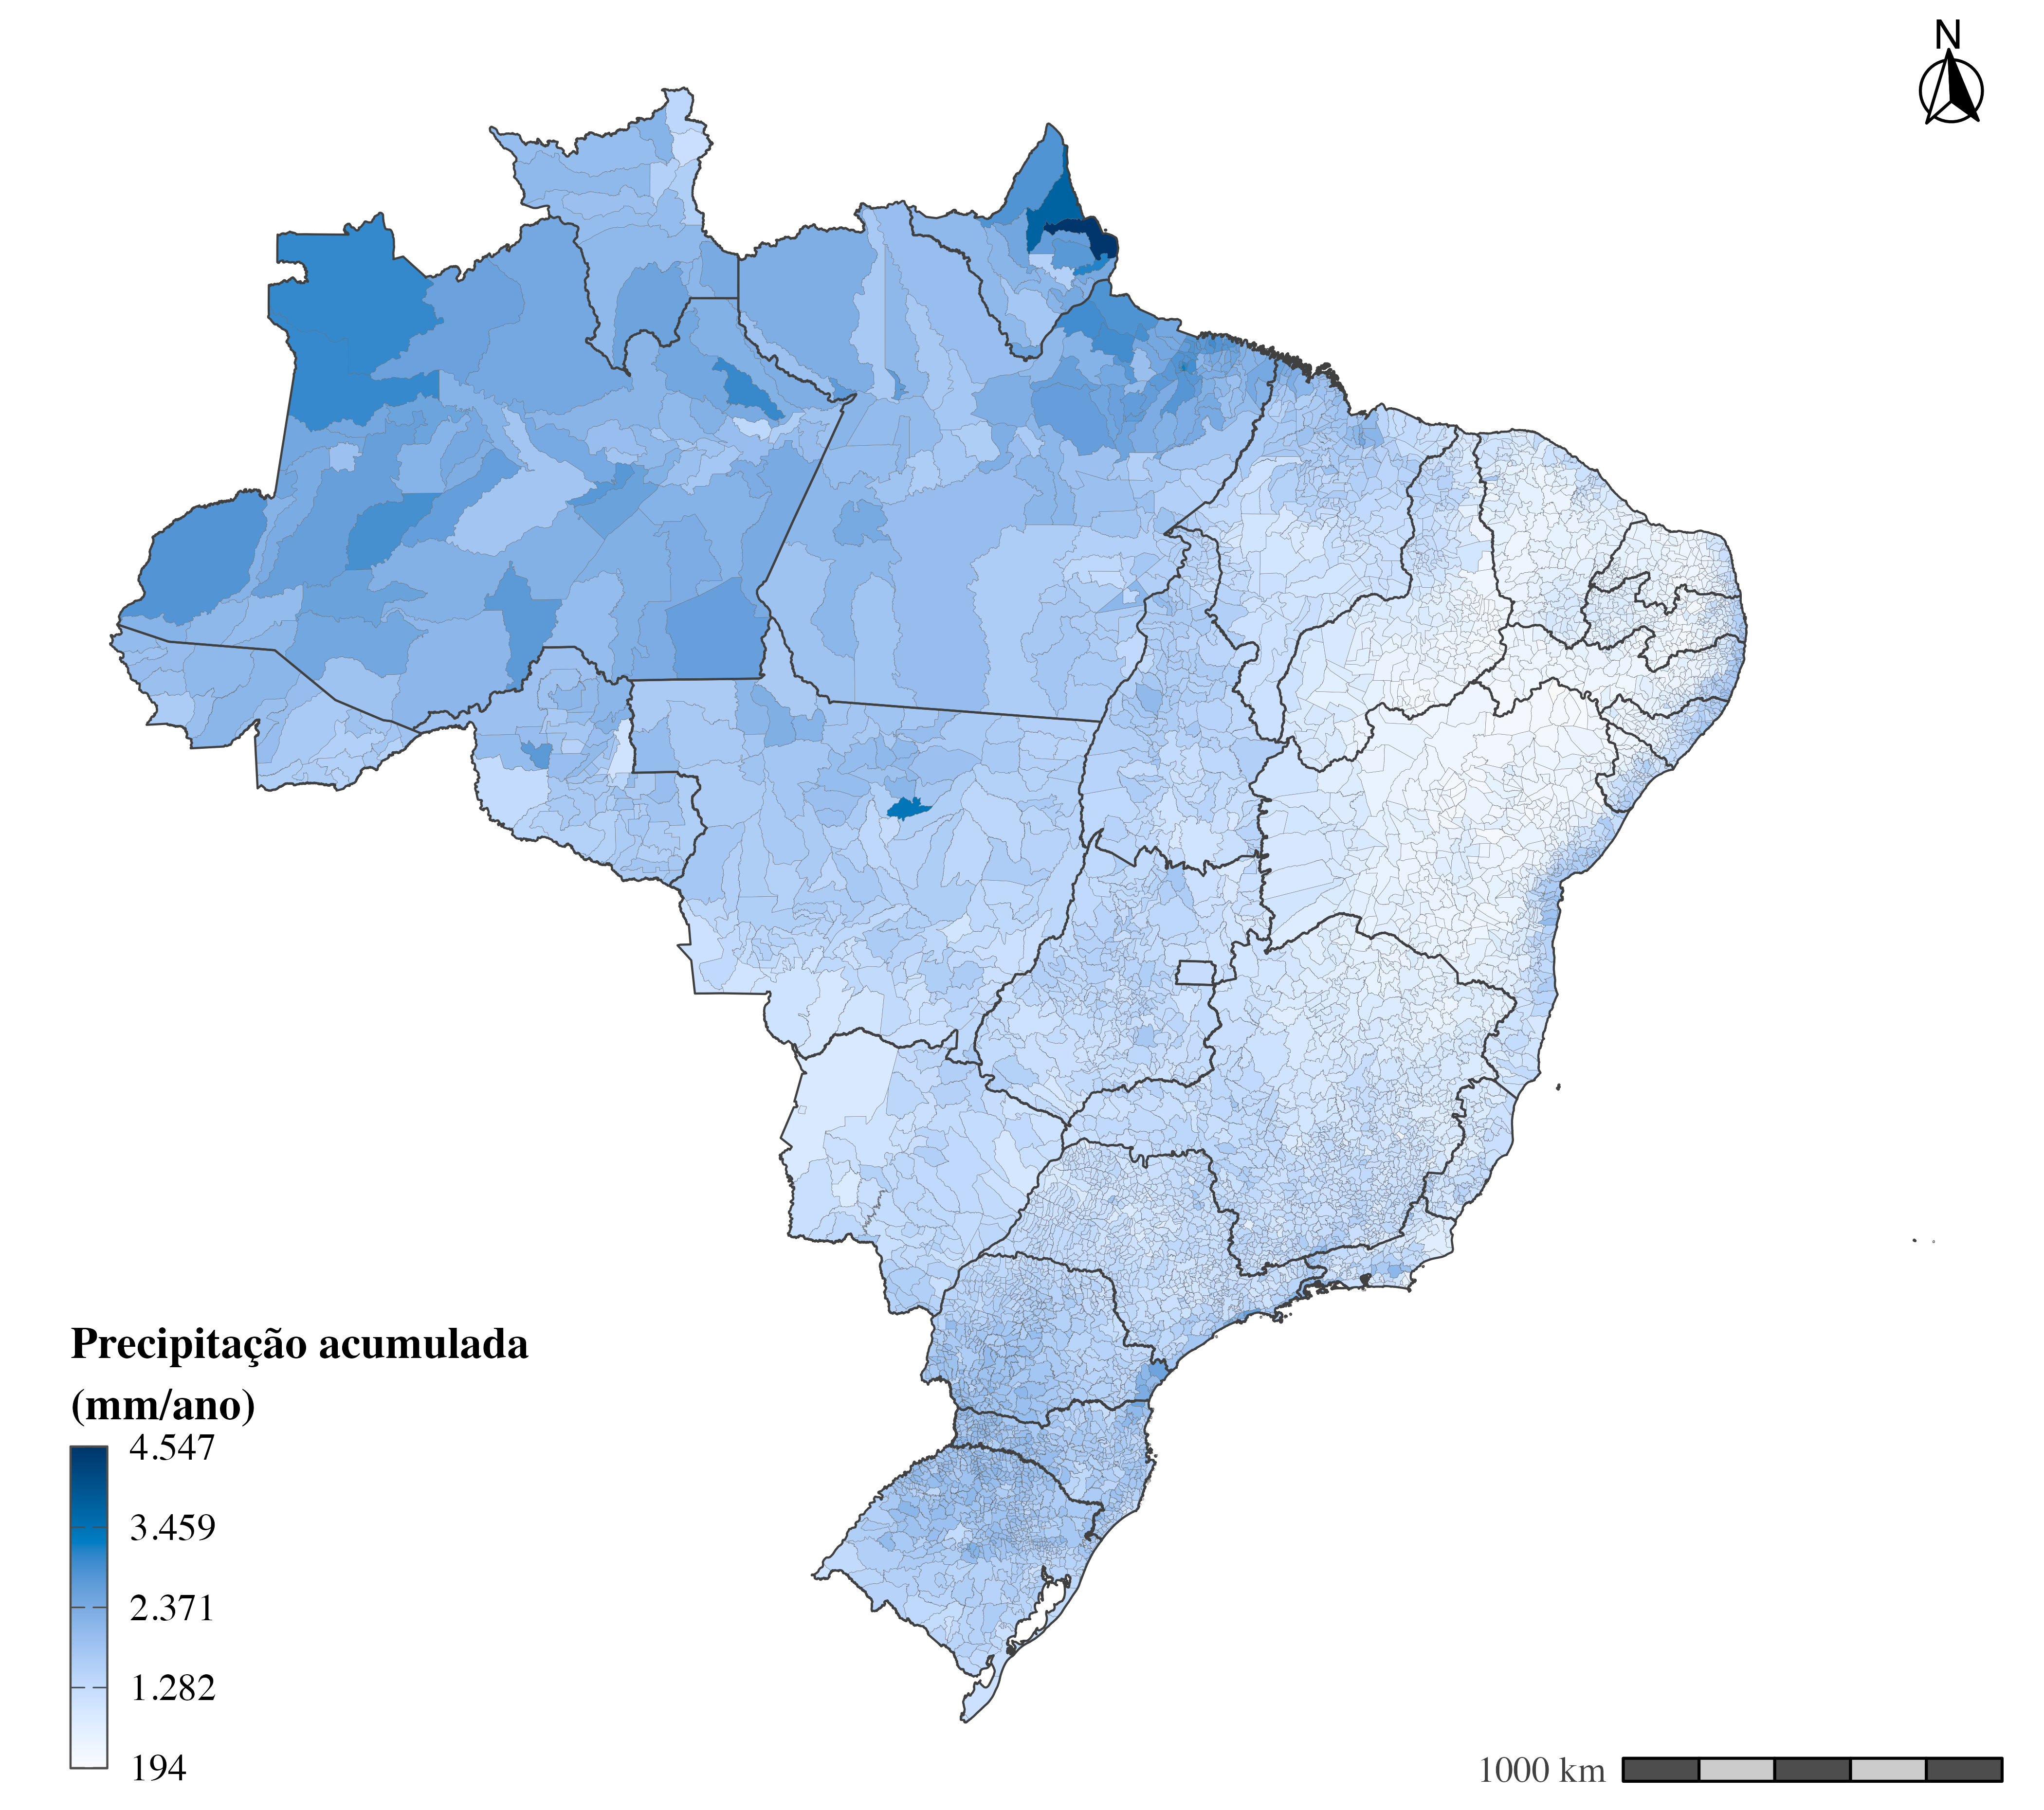
\includegraphics[width=0.64\textwidth]{fig_mapa_precipitacao.png}
    \caption{Precipitação anual acumulada por município, Brasil, 2010--2025, em milímetros por ano. Fonte: estações de superfície.}
    \label{fig:mapa_precipitacao}
\end{figure}

\begin{figure}[H]
    \centering
    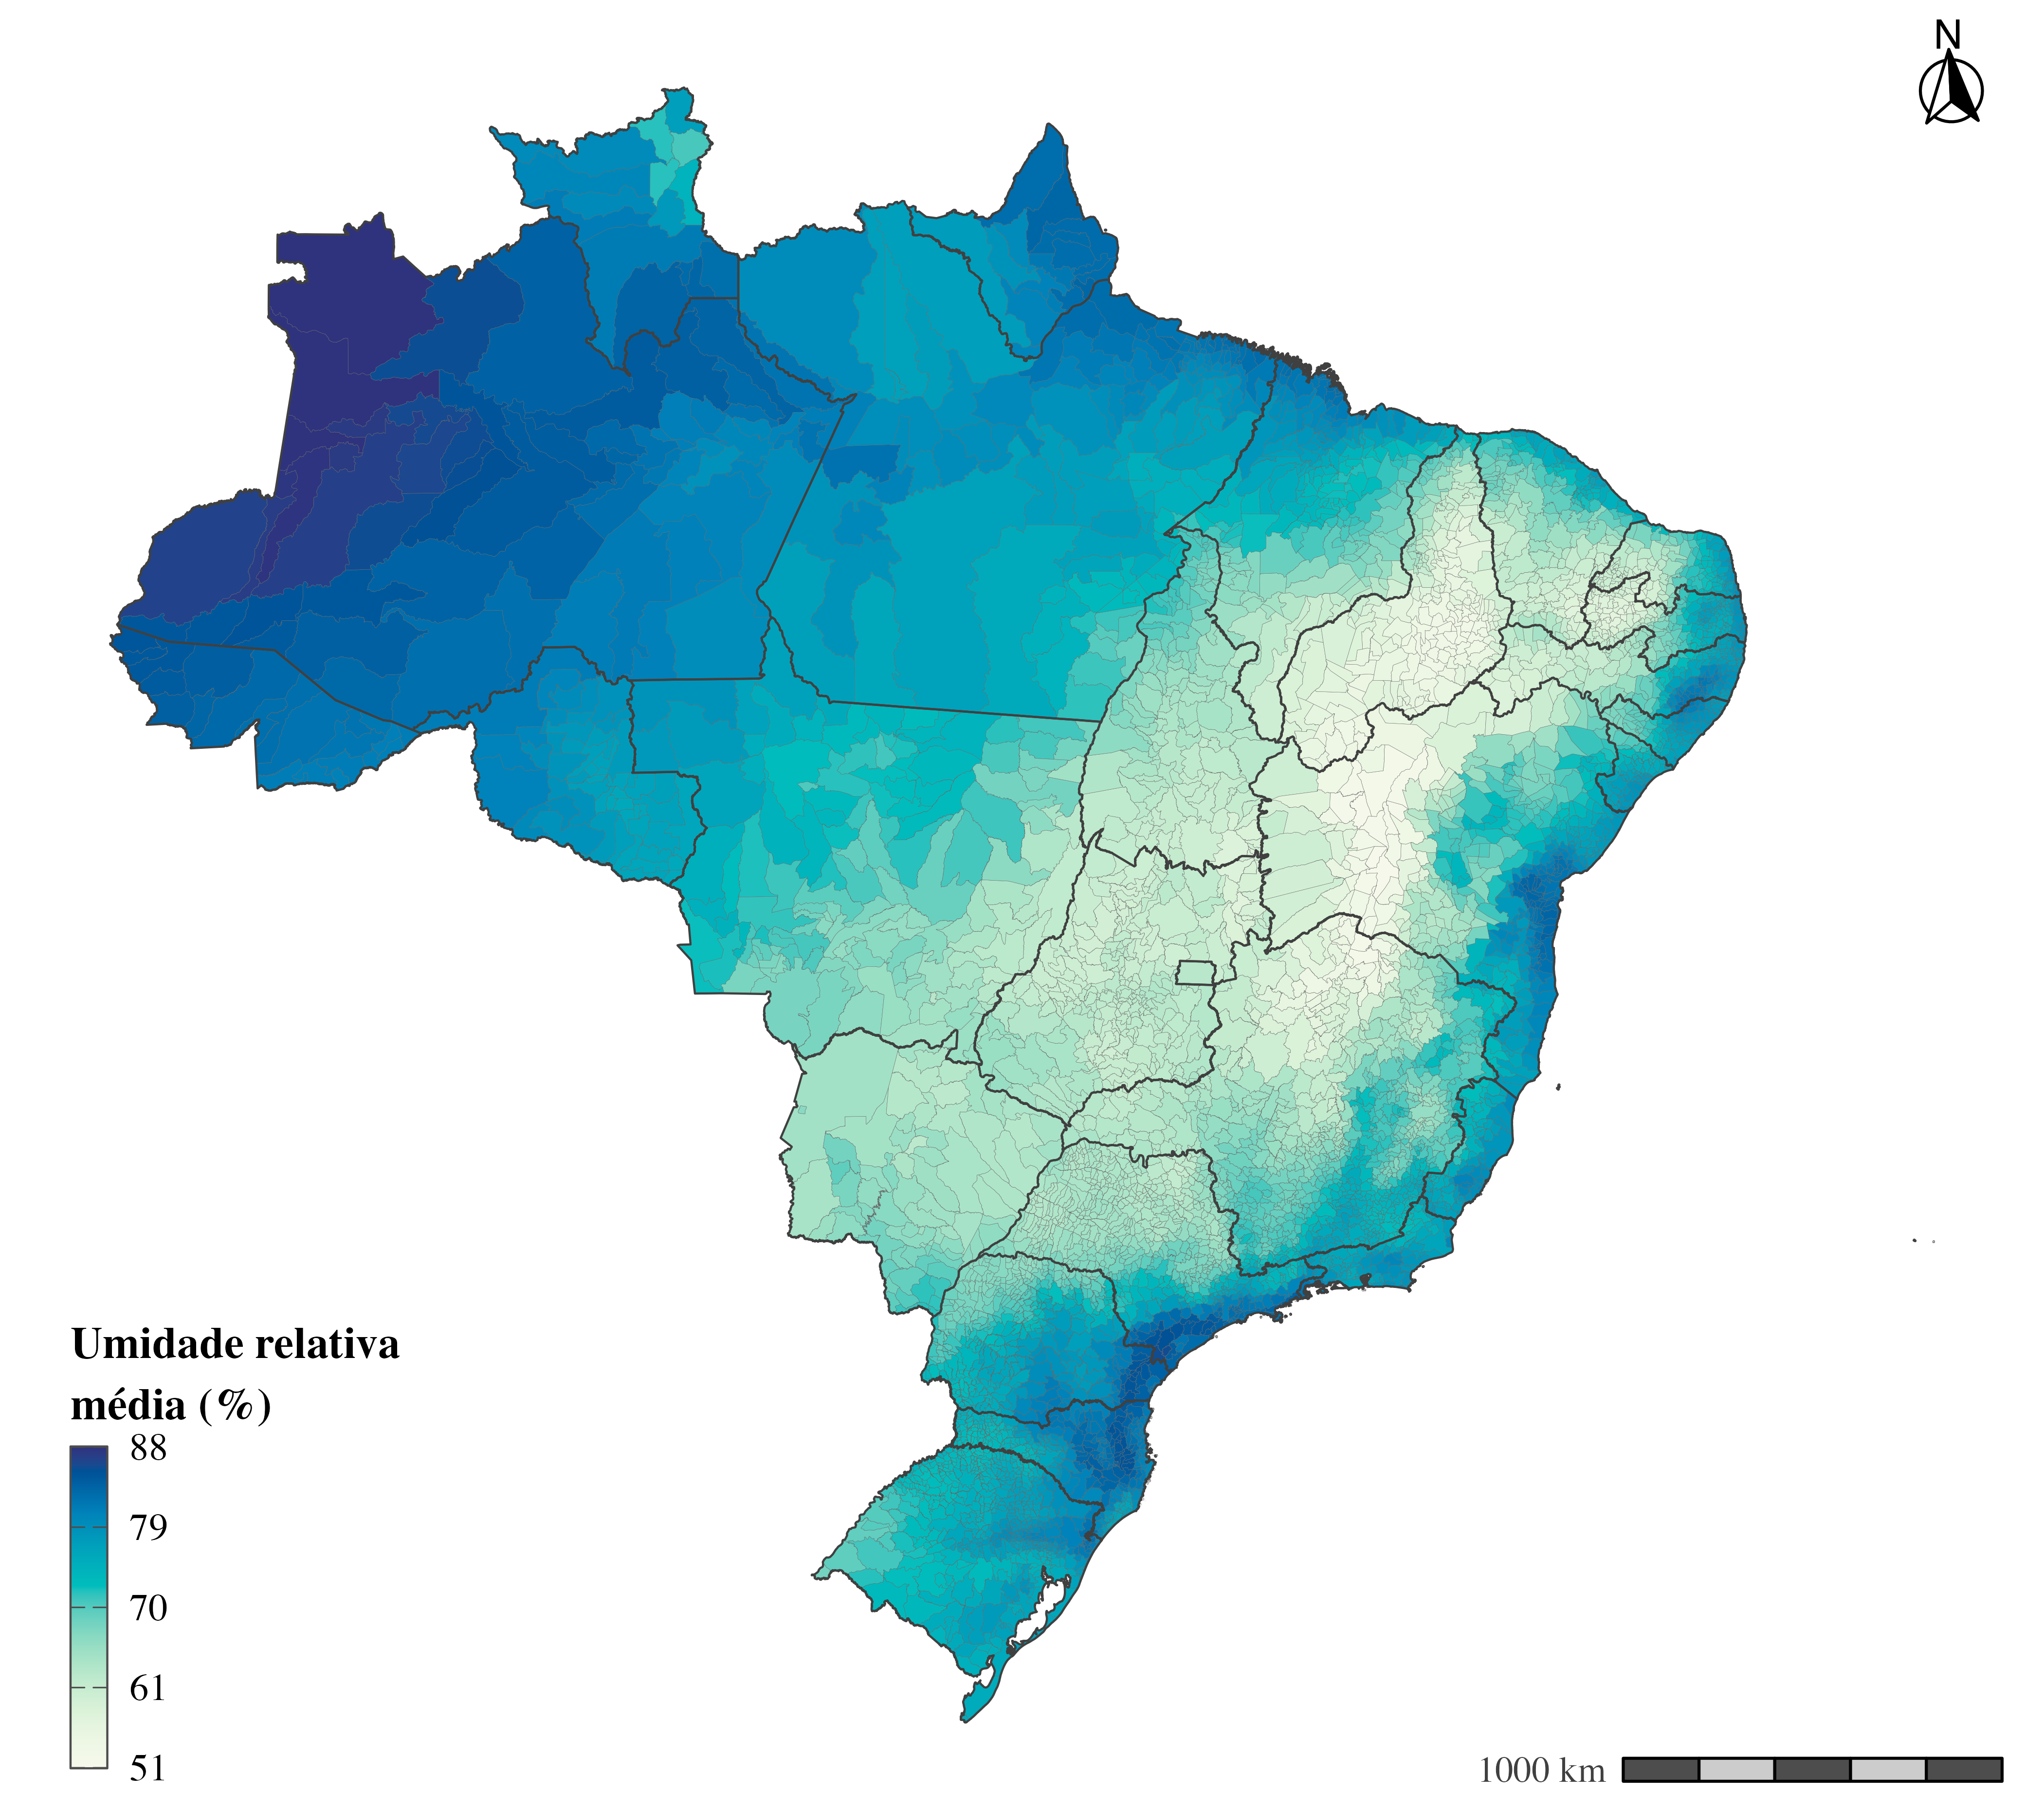
\includegraphics[width=0.64\textwidth]{fig_mapa_umidade.png}
    \caption{Média municipal da umidade relativa do ar, Brasil, 2010--2025, em percentual. Fonte: reanálise climática.}
    \label{fig:mapa_umidade}
\end{figure}

A variação mensal da temperatura acompanha o padrão descrito na Tabela~\ref{tab:resumo_clima}, com medianas mais altas no verão e mais baixas no inverno (Figura~\ref{fig:serie_boxplot_temperatura}).

\begin{figure}[H]
    \centering
    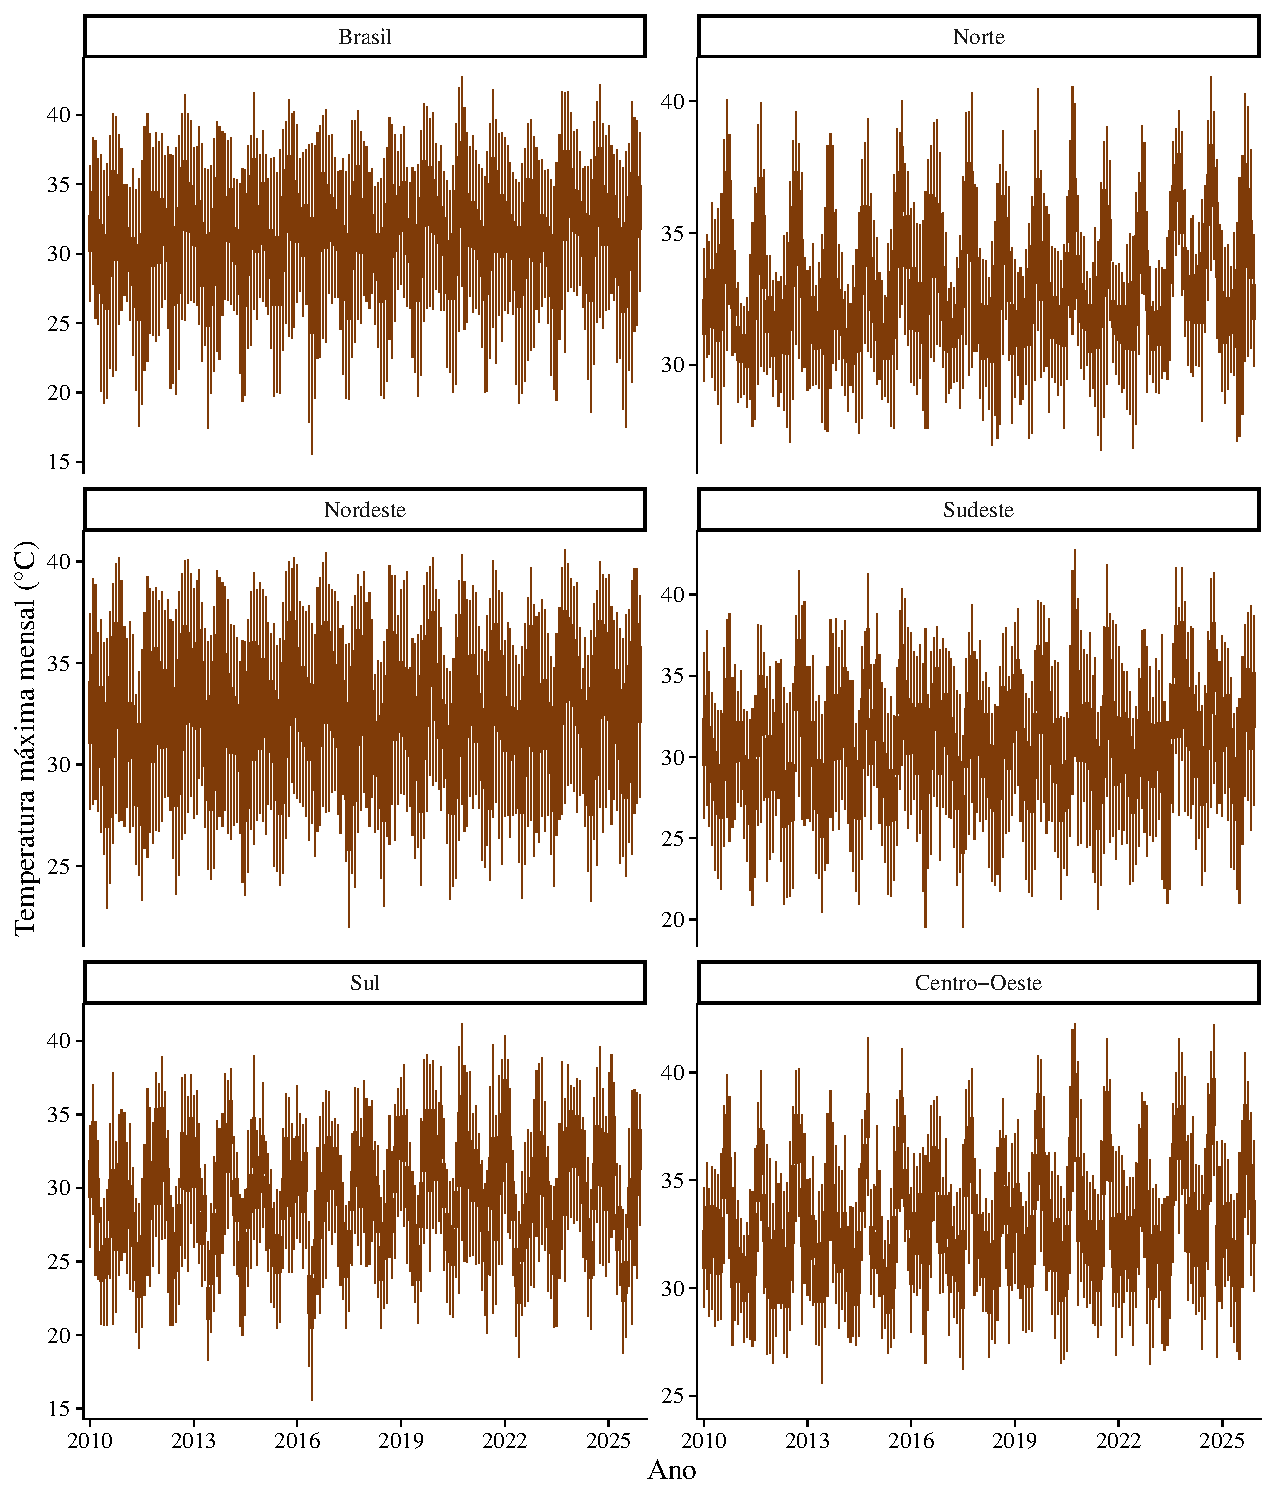
\includegraphics[width=0.95\textwidth]{fig_serie_boxplot_temperatura.pdf}
    \caption{Série mensal da temperatura máxima por Grande Região, Brasil, 2010--2025, em graus Celsius, com distribuição municipal resumida por mês. Fonte: reanálise climática.}
    \label{fig:serie_boxplot_temperatura}
\end{figure}

\subsection{Estratificação de risco e persistência epidêmica}
\label{subsec:resultados_estratificacao}

A Tabela~\ref{tab:estratificacao_risco} apresenta a distribuição dos \NumMunicipios{} municípios pelos estratos definidos para a razão acumulada de casos por população média: baixa (menos de 100 casos por 100 mil habitantes), média (100 a 300) e alta (mais de 300). No agregado nacional, \PctMunAltoRisco{} dos municípios ficaram no estrato alto, \PctMunMedioRisco{} no médio e \PctMunBaixoRisco{} no baixo. Nas regiões Sudeste e Centro-Oeste, praticamente todos os municípios enquadraram-se no estrato alto (99,9\% e 100,0\%, respectivamente), enquanto o Sul concentrou os de menor razão acumulada.

\begin{table}[!h]
\centering
\caption{\label{tab:estratificacao_risco}Distribuição dos municípios por estrato de risco e Grande Região, Brasil, 2010--2025.}
\centering
\resizebox{\ifdim\width>\linewidth\linewidth\else\width\fi}{!}{
\fontsize{9}{11}\selectfont
\begin{tabular}[t]{lcccccc}
\toprule
Estrato & Brasil & Norte & Nordeste & Sudeste & Sul & Centro-Oeste\\
\midrule
Baixa & 114 (2,0\%) & 8 (1,8\%) & 6 (0,3\%) & 0 (0,0\%) & 100 (8,4\%) & 0 (0,0\%)\\
Média & 254 (4,6\%) & 20 (4,5\%) & 42 (2,3\%) & 1 (0,1\%) & 191 (16,1\%) & 0 (0,0\%)\\
Alta & 5.196 (93,4\%) & 421 (93,8\%) & 1.745 (97,3\%) & 1.667 (99,9\%) & 897 (75,5\%) & 466 (100,0\%)\\
\bottomrule
\end{tabular}}
\end{table}


Na estratificação por tercis, as taxas por 100 mil pessoas-ano nos níveis 1 a 3 foram 797,6, 483,5 e 357,5 para esgotamento adequado; 821,7, 502,5 e 311,7 para abastecimento de água por rede; e 779,0, 526,8 e 305,5 para coleta de lixo. Para a densidade urbana, a taxa foi maior no nível intermediário (613,1; 768,4; e 649,2), enquanto para a proporção urbana aumentou entre os níveis (436,5; 558,3; e 732,8). Esses contrastes são descritivos e não estimam efeitos das covariáveis.

A Figura~\ref{fig:mapa_incidencia} apresenta a razão acumulada de casos por população média no período. \PctMunPersistencia{} dos municípios apresentaram dez ou mais anos com taxa anual acima de 300 por 100 mil habitantes, persistência mostrada na Figura~\ref{fig:mapa_persistencia}.

\begin{figure}[H]
    \centering
    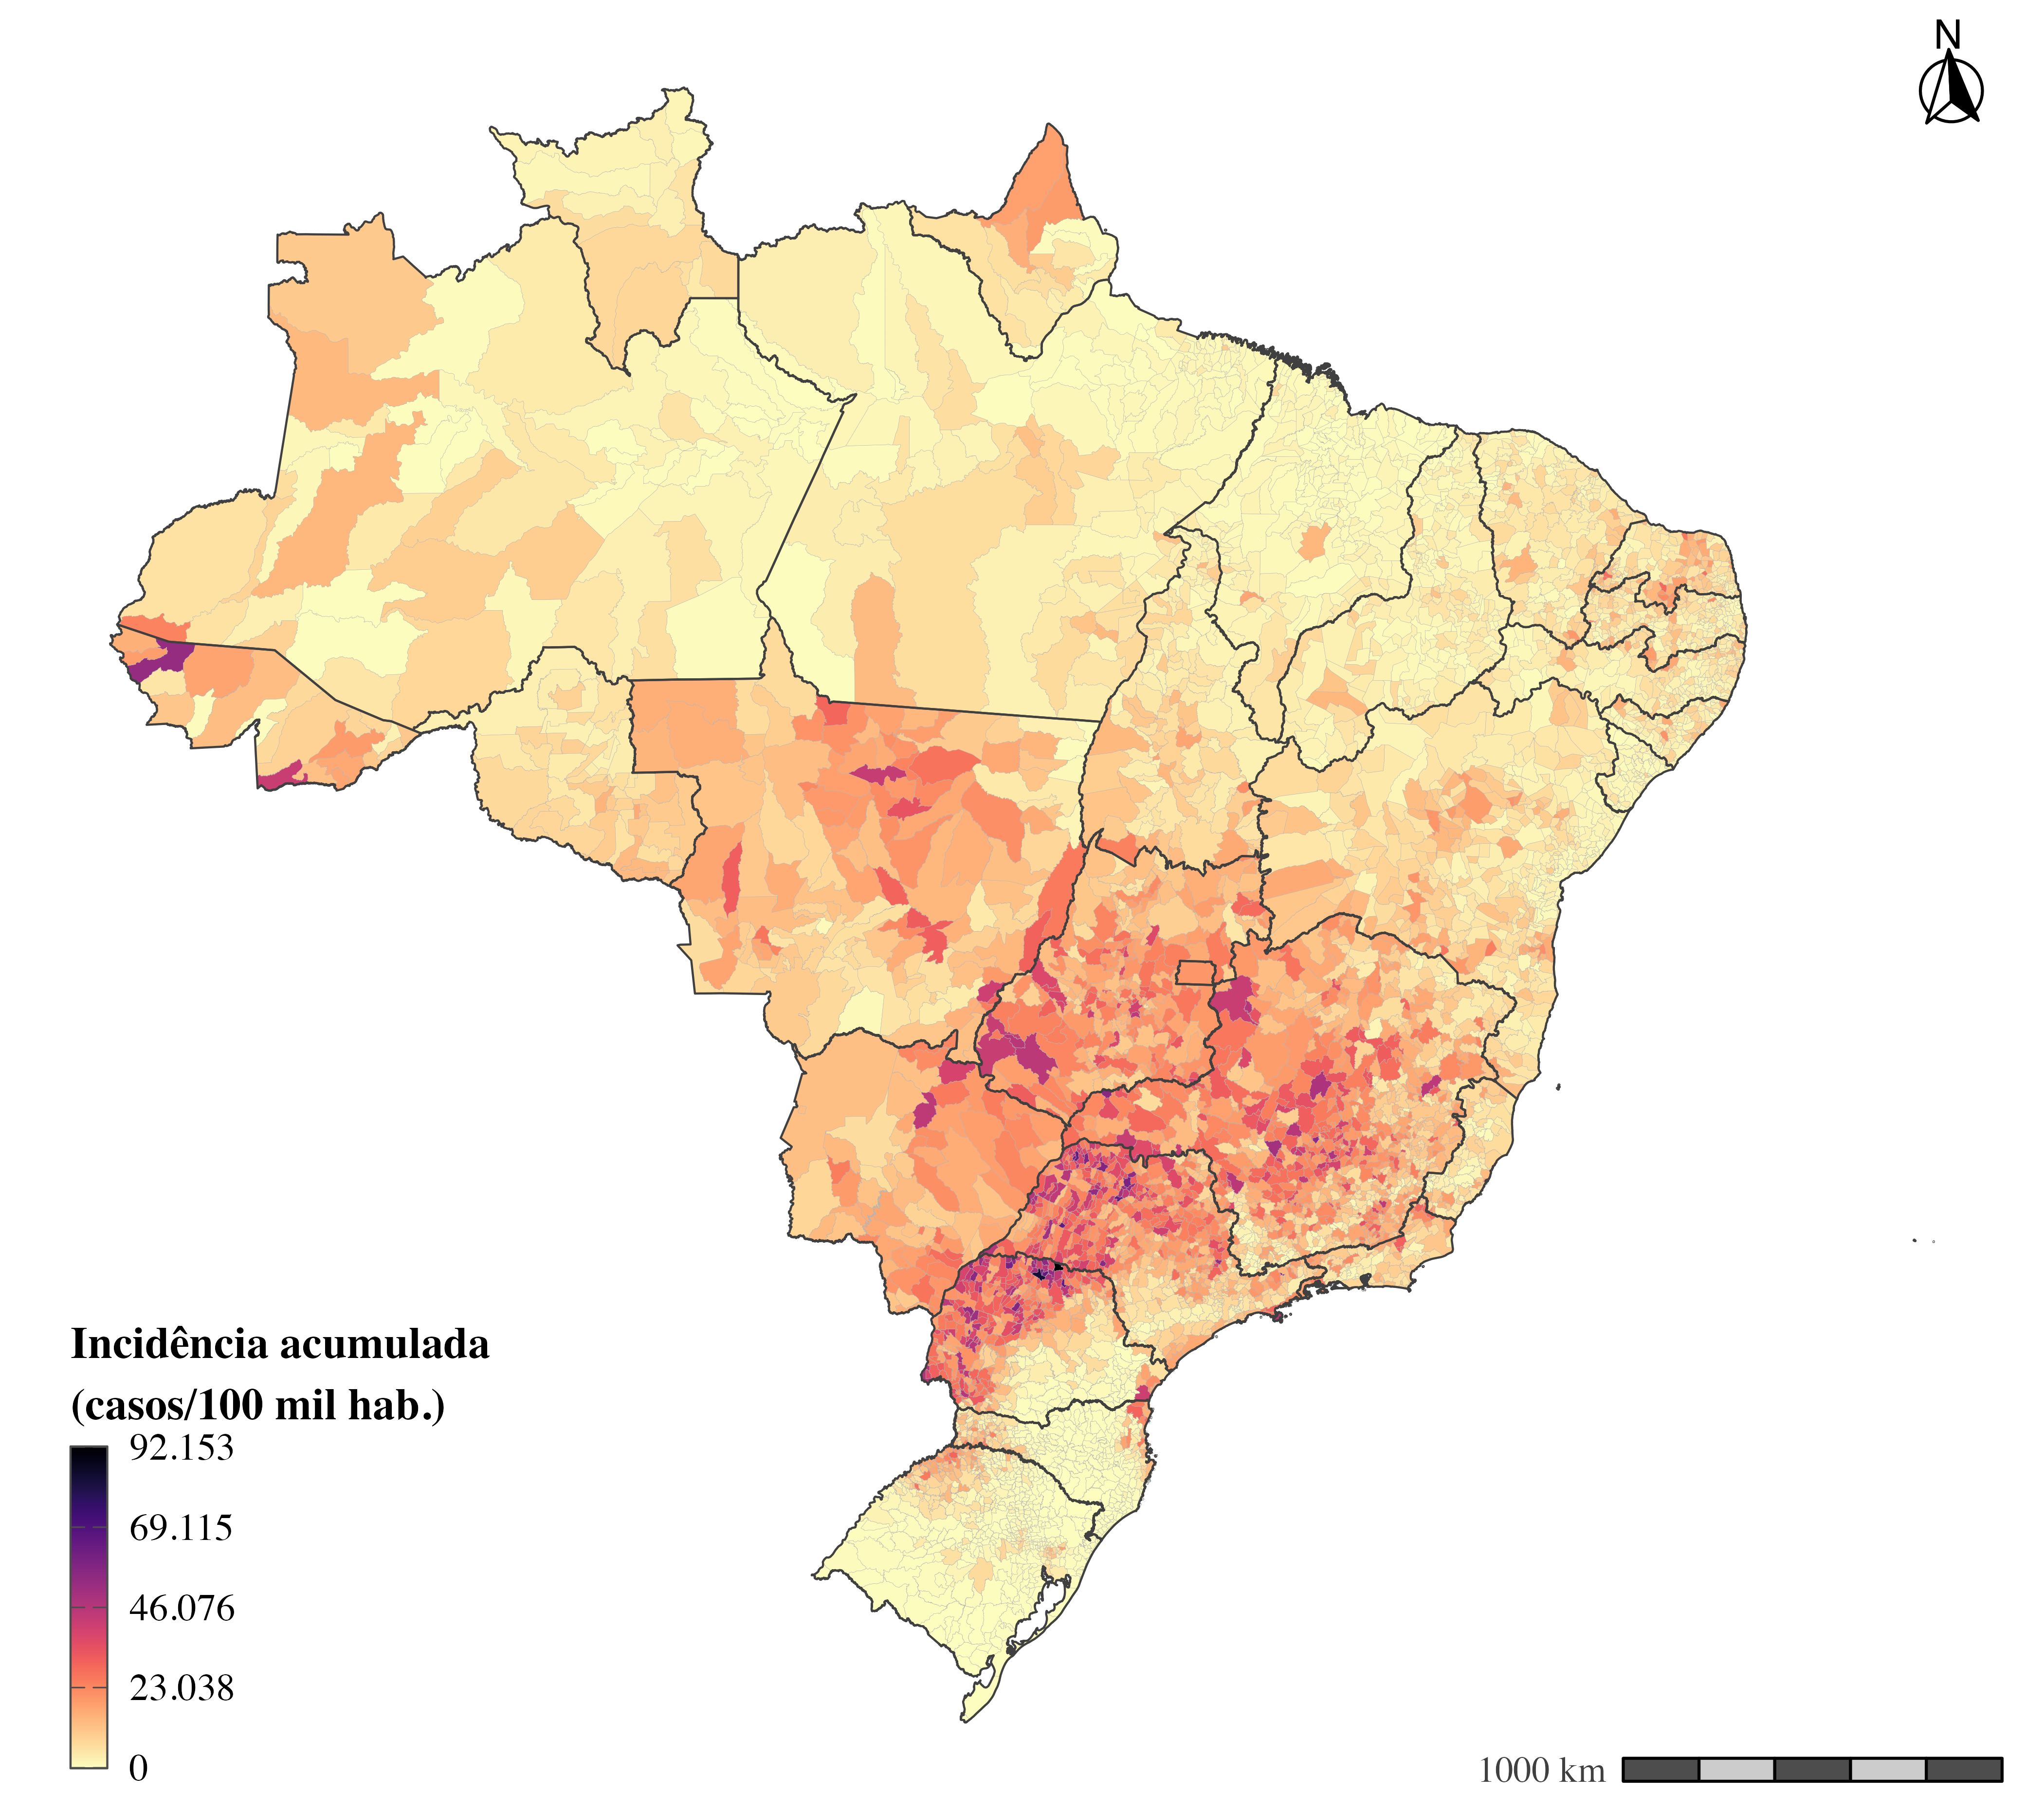
\includegraphics[width=0.76\textwidth]{fig_mapa_incidencia_acumulada.png}
    \caption{Razão acumulada de casos prováveis de dengue por população média municipal, Brasil, 2010--2025, expressa por 100 mil habitantes. Fontes: SINAN e IBGE.}
    \label{fig:mapa_incidencia}
\end{figure}

\begin{figure}[H]
    \centering
    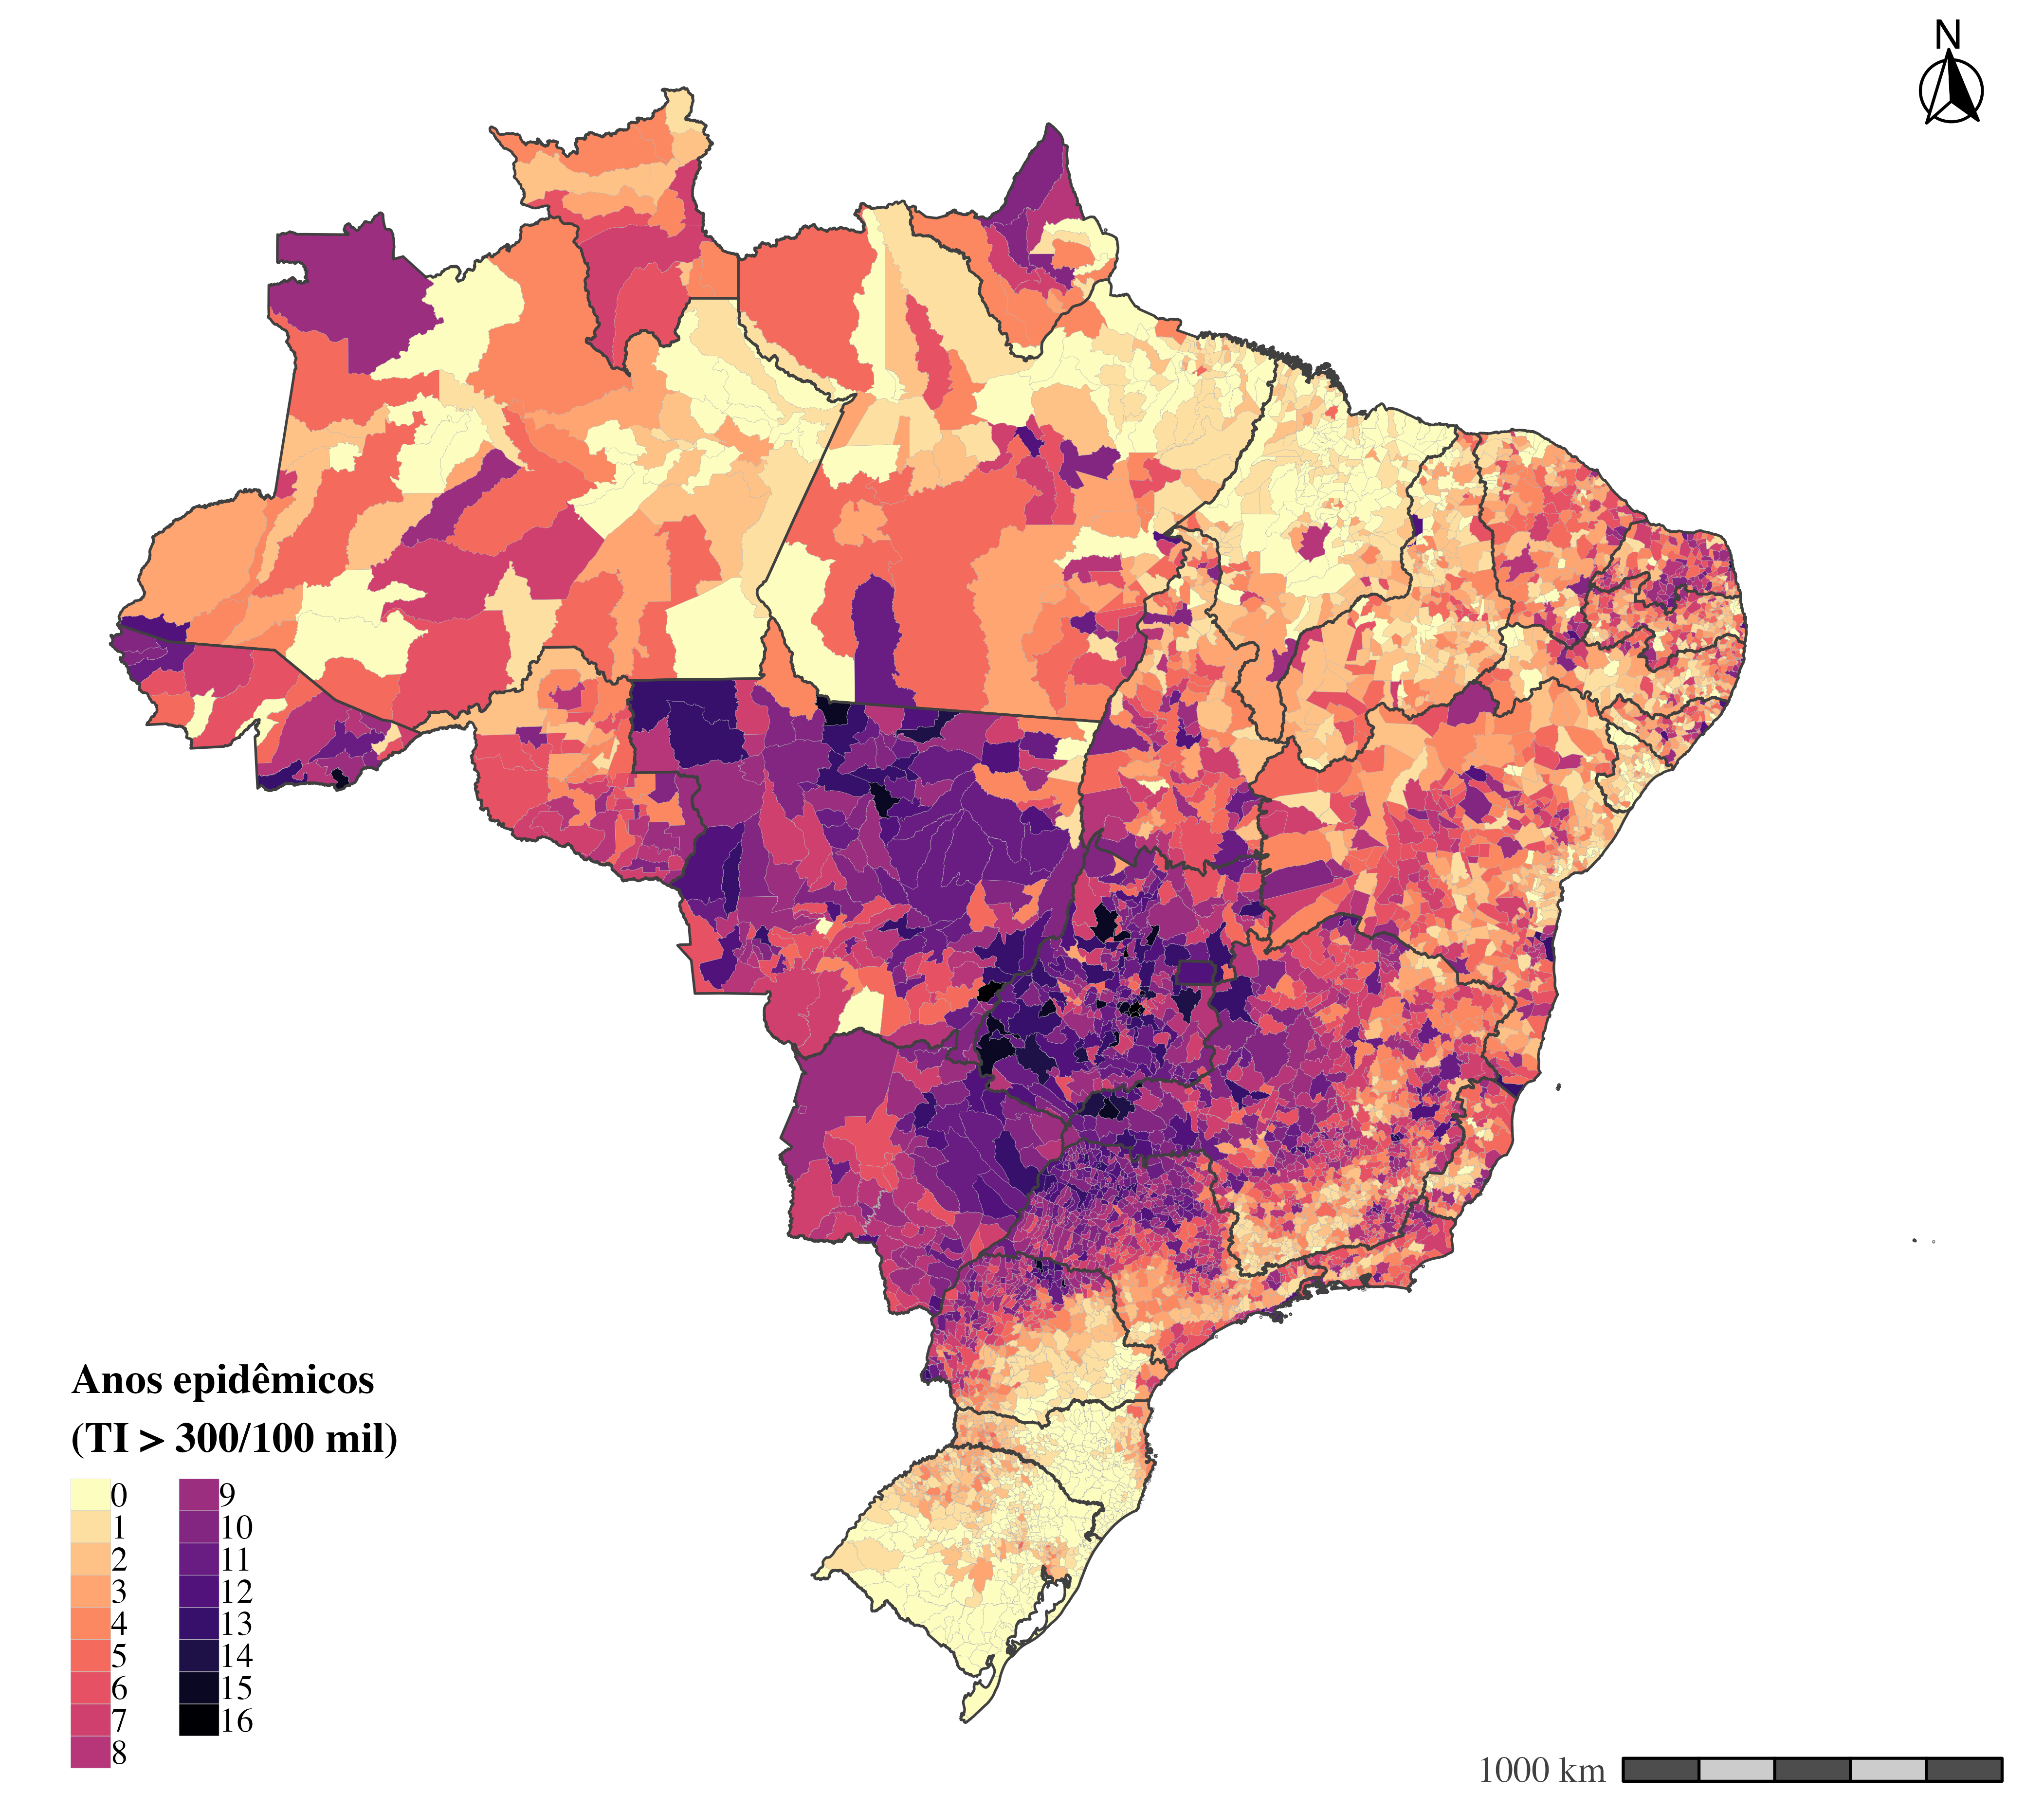
\includegraphics[width=0.76\textwidth]{fig_mapa_persistencia_epidemica.png}
    \caption{Número de anos, entre 2010 e 2025, com taxa de incidência acima de 300 casos por 100 mil habitantes, por município, Brasil. Fontes: SINAN e IBGE.}
    \label{fig:mapa_persistencia}
\end{figure}

Os quadrantes locais (Figura~\ref{fig:mapa_lisa}) mostram \textit{clusters} alto-alto entre Centro-Oeste e Sudeste e \textit{clusters} baixo-baixo na Amazônia Ocidental, em faixas do interior do Nordeste e no extremo Sul. A parcela sem associação local significativa foi de \LisaPctNS{}; a seção seguinte busca zonas de risco elevado pela estatística de varredura.

\section{Detecção e Análise de \textit{Clusters} Espaciais}
\label{sec:clusters}

A varredura espacial usou os \ScanTotalCasos{} casos do painel e a população média residente (\ScanPopulacao{} habitantes). Os casos de 2024 representam 29,1\% do total acumulado, de modo que a varredura reflete esse ano epidêmico. A comparação entre as oito formulações é descritiva e exploratória: o método delimita zonas de excesso, e não estima efeitos como uma regressão. Antes da apresentação detalhada dos \textit{clusters}, o modelo sem ajuste e os sete ajustes são confrontados quanto ao número e à posição das zonas, ao erro absoluto percentual ponderado e à sobreposição municipal; essa comparação orienta a leitura das subseções seguintes.

\subsection{Comparação entre as oito formulações}
\label{subsec:satscan_sensibilidade}

Cada formulação gerou uma coleção própria de zonas e uma distribuição própria de casos esperados municipais. A Tabela~\ref{tab:comparacao_satscan} resume os resultados. As coleções variaram de 128 (calor) a 195 (lixo) zonas significativas, com cobertura entre 62,5\% e 64,9\% dos casos do painel. O polo primário permaneceu no Centro-Sul em todas as formulações, com deslocamento entre Adolfo (SP) no modelo sem ajuste, Queluzito (MG) sob calor, Iacri (SP) sob esgoto, proporção urbana, água e lixo, e Araújos (MG) sob densidade urbana e índice composto. O WMAPE, que resume a proximidade entre esperado padronizado e observado, caiu de 75,1\% sem ajuste para 64,9\% sob calor, 70,5\% sob água, 71,9\% sob esgoto, 71,9\% sob o índice composto, 72,1\% sob lixo, 74,3\% sob densidade urbana e 74,4\% sob proporção urbana. A sobreposição municipal com o modelo sem ajuste (índice de Jaccard) ficou entre 56\% (calor) e 82\% (densidade urbana). Em nenhuma formulação a redução do WMAPE foi acompanhada do desaparecimento das zonas de excesso.

\begin{table}[!h]
\centering
\caption{\label{tab:comparacao_satscan}Comparação dos ajustes por covariáveis na varredura espacial: zonas significativas, polo primário, risco relativo, cobertura de casos e WMAPE nacional, Brasil, 2010--2025.}
\centering
\resizebox{\ifdim\width>\linewidth\linewidth\else\width\fi}{!}{
\fontsize{9}{11}\selectfont
\begin{tabular}[t]{lclcccc}
\toprule
Ajuste & Zonas & Primário (polo) & $RR$ & \% dos casos & WMAPE (\%) & Redução (p.p.)\\
\midrule
Sem ajuste & 129 & Adolfo (SP) & 2,99 & 64,1\% & 75,1 & —\\
Calor & 128 & Queluzito (MG) & 2,08 & 63,3\% & 64,9 & 10,2\\
Esgoto adequado & 178 & Iacri (SP) & 2,79 & 64,0\% & 71,9 & 3,2\\
Densidade urbana & 136 & Araújos (MG) & 2,73 & 63,2\% & 74,3 & 0,8\\
Proporção urbana & 158 & Iacri (SP) & 3,11 & 63,3\% & 74,4 & 0,6\\
\addlinespace
Água por rede & 193 & Iacri (SP) & 2,70 & 63,4\% & 70,5 & 4,6\\
Coleta de lixo & 195 & Iacri (SP) & 2,86 & 64,9\% & 72,1 & 3,0\\
Índice composto & 184 & Araújos (MG) & 2,58 & 62,5\% & 71,9 & 3,2\\
\bottomrule
\end{tabular}}
\end{table}


O ajuste por tercis de dias em onda de calor combinou a maior redução do WMAPE (de 75,1\% para 64,9\%, 10,2 pontos percentuais) com a manutenção de uma coleção extensa de zonas residuais, razão pela qual as subseções seguintes detalham o modelo sem ajuste e o ajuste por calor.

\subsection{Consistência das zonas entre as formulações}

Para resumir a robustez das zonas às diferentes estratificações, a Figura~\ref{fig:robustez} classifica cada município pelo número de formulações (o modelo sem ajuste e os sete ajustes, de uma a oito) em que ele pertence a uma zona significativa, sobrepondo as coleções de todos os modelos. Dos 5.564 municípios do painel, 3.016 (54,2\%) aparecem em pelo menos uma formulação, 1.655 (29,7\%) em seis ou mais e 967 (17,4\%) em todas as oito; 378 municípios aparecem em apenas uma. Os tons mais escuros concentram-se no Centro-Sul, sobretudo no Sudeste e no Centro-Oeste, enquanto a maior parte do Norte e do interior do Nordeste permanece fora de zonas ou em poucas formulações. A leitura é de robustez às formulações, e não de intensidade de risco: aparecer em todas elas indica que o excesso se mantém sob qualquer um dos esquemas de padronização testados, ao passo que aparecer em poucas acompanha os excessos marginais descritos no modelo sem ajuste. 
\begin{figure}[H]
    \centering
    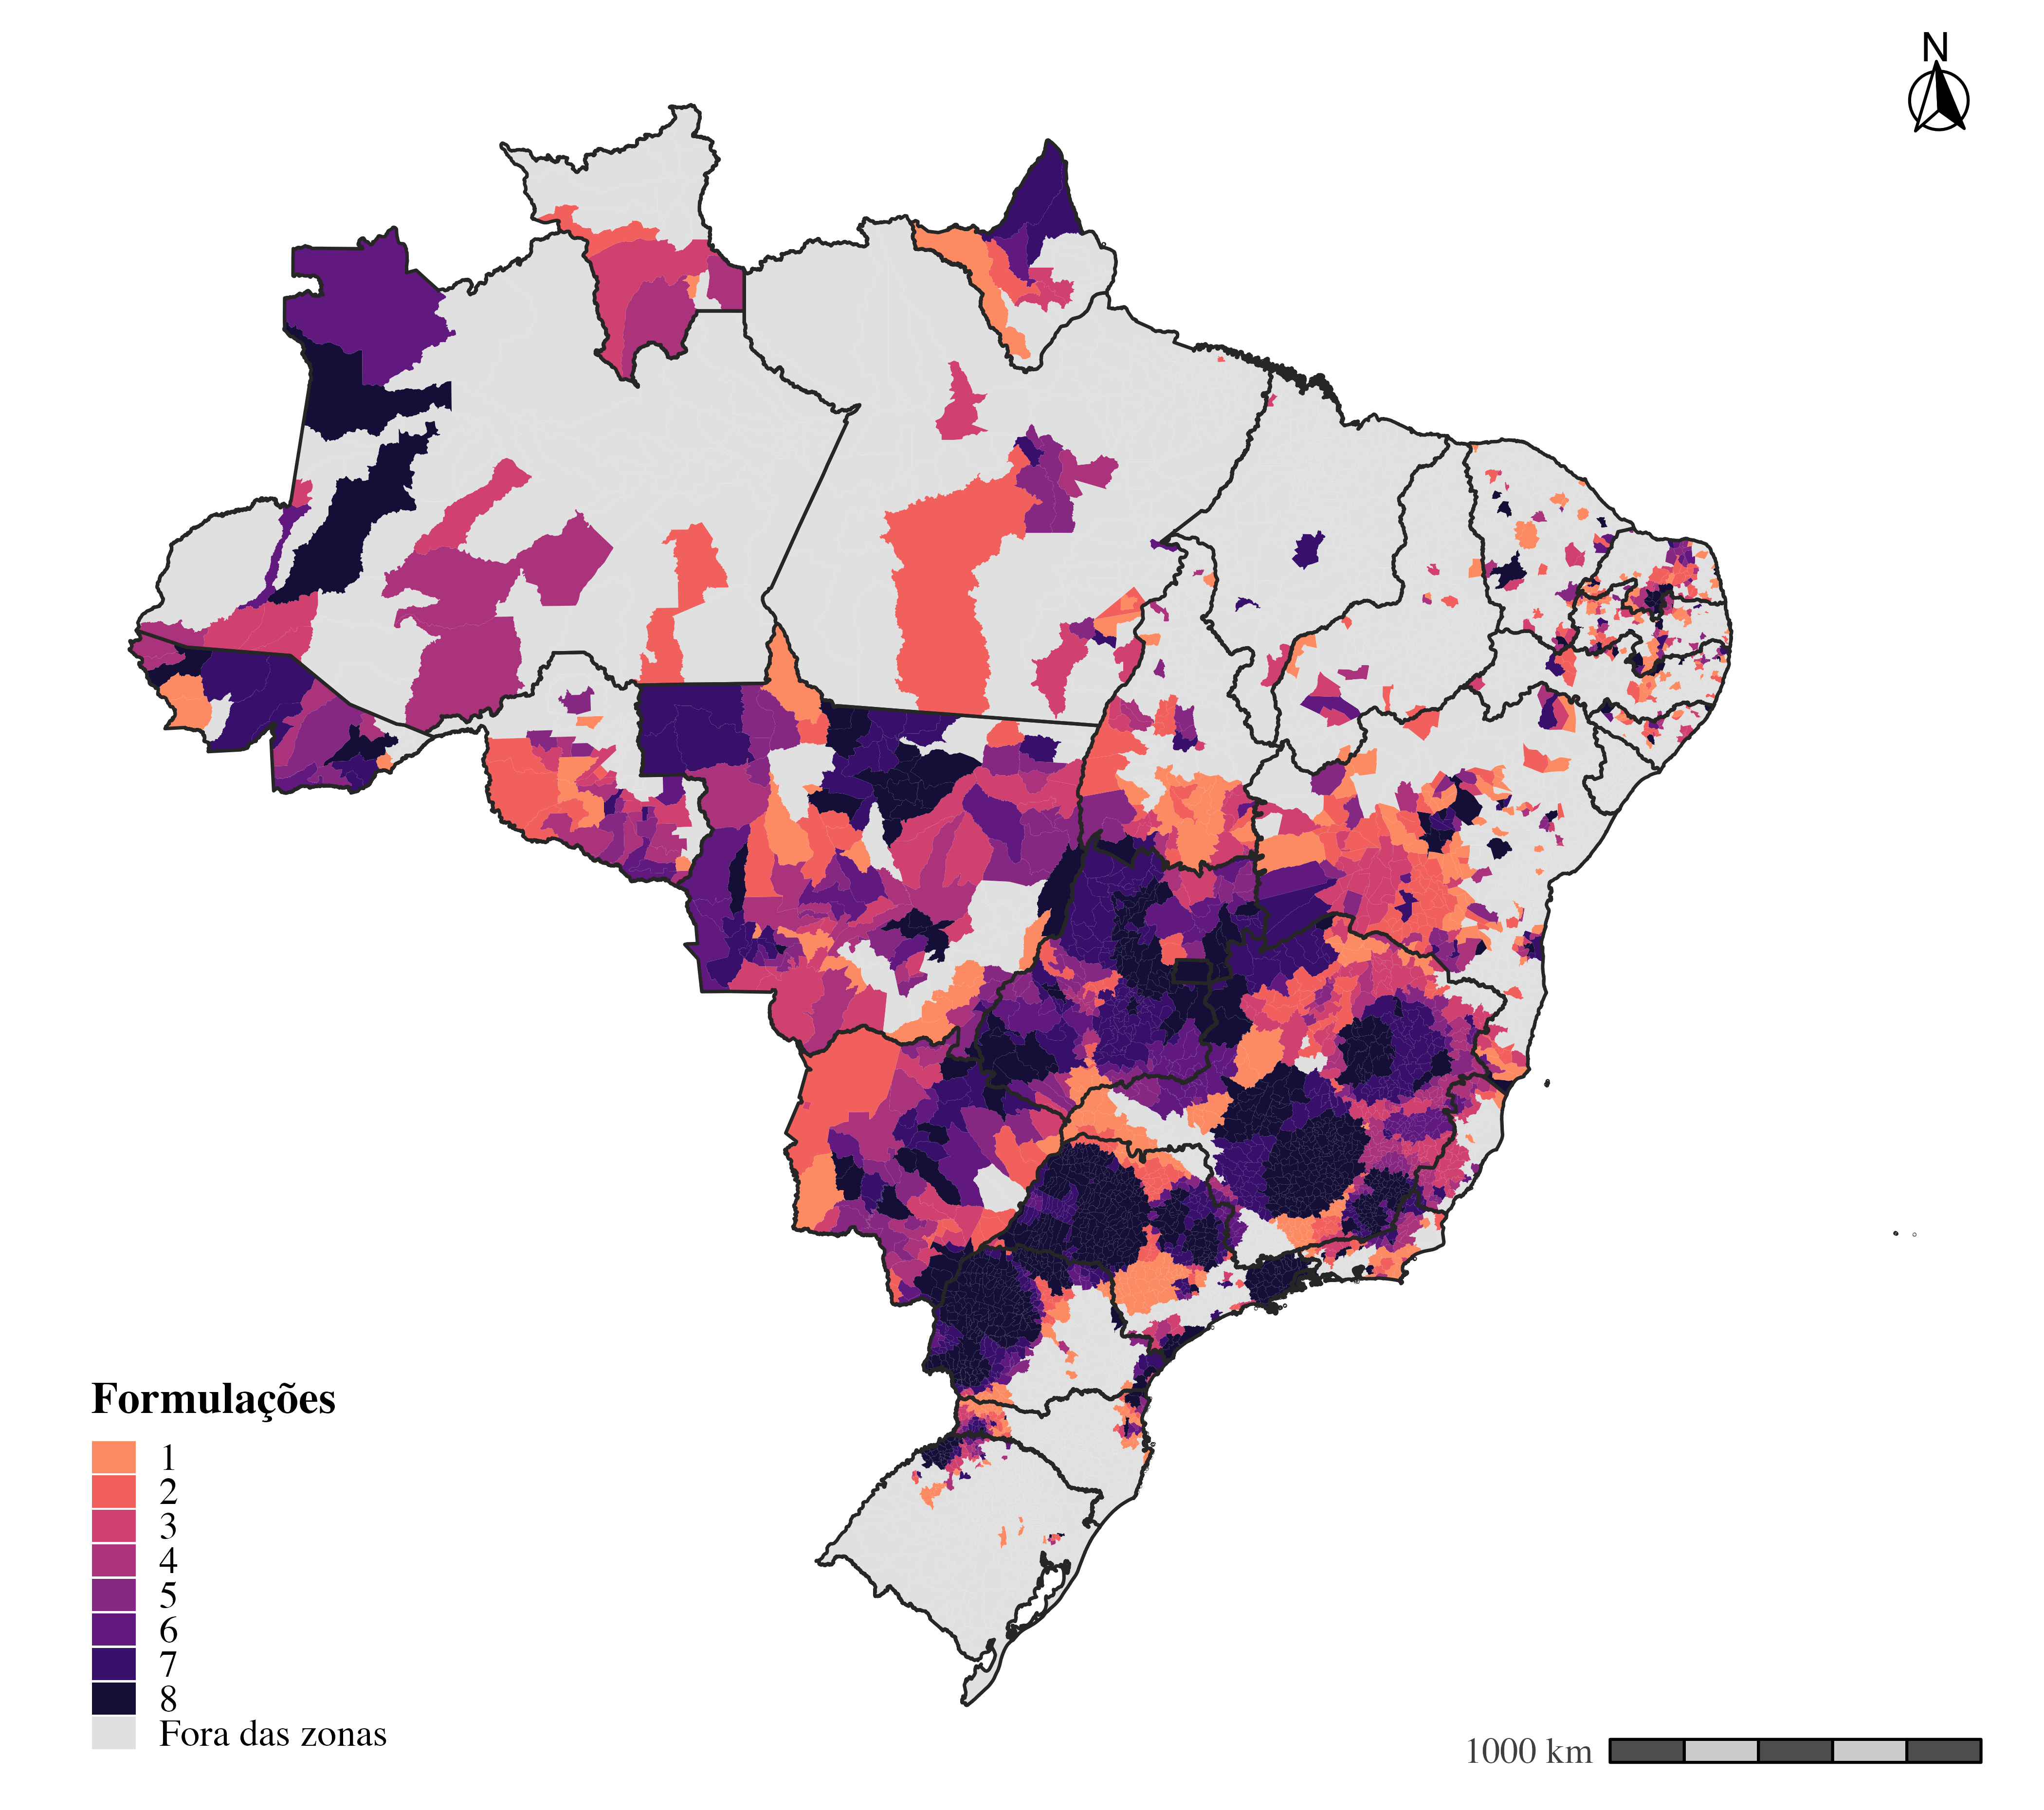
\includegraphics[width=0.76\textwidth]{fig_mapa_persistencia_ajustes.png}
    \caption{Consistência das zonas significativas de alto risco entre as formulações da varredura espacial, Brasil, 2010--2025: número de formulações, de uma a oito, em que cada município pertence a uma zona. Fontes: SINAN e IBGE.}
    \label{fig:robustez}
    \vspace{0.3em}
    {\footnotesize\noindent\textit{Nota:} Tons mais escuros indicam presença em mais formulações, no gradiente discreto de uma a oito; em cinza, municípios que não pertencem a zonas em nenhuma das oito formulações.\par}
\end{figure}

\subsection{Modelo sem ajuste}
\label{subsec:satscan_puro}

Com limite de 16\% da população e 200~km de raio, o modelo sem ajuste reteve 129 zonas sem sobreposição (nível de 5\%), que recobriram \ScanCobMunicipios{} municípios (\ScanCobMunicipiosPct{} dos municípios) e concentraram \ScanCobCasos{} casos (\ScanCobCasosPct{} dos casos do painel) em \ScanCobPopPct{} da população sob risco. Das 129 zonas significativas, 16 apresentam risco relativo abaixo de 1,2 e 70 abaixo de 1,5, de modo que parte da coleção corresponde a excessos marginais\footnote{Isto é, zonas cujo risco relativo é pouco maior que 1; a significância dessas zonas decorre sobretudo do volume acumulado sob o modelo de Poisson.}. A Figura~\ref{fig:mapas_zonas} mostra a extensão dessas zonas (painel a) e a coleção do ajuste por calor (painel b), para comparação; a Figura~\ref{fig:mapas_rr} usa os mesmos dois modelos para o risco relativo municipal.

O \textit{cluster} primário centrou-se em Adolfo (SP), com \ScanPrimMunicipios{} municípios em um raio de \ScanPrimRaioKm{}~km, \ScanPrimCasosObs{} casos observados contra \ScanPrimCasosEsp{} esperados, risco relativo de $RR = \ScanPrimRR{}$ ($p \ScanPrimPValor{}$; razão de verossimilhança logarítmica (LLR) $= \ScanPrimLLR{}$), abrangendo \ScanPrimPop{} habitantes (\ScanPrimPopPct{} da população) e \ScanPrimCasosPct{} dos casos. O segundo aglomerado centrou-se em Araújos (MG), com 229 municípios em raio de 199,8~km ($RR = 2{,}74$; 2.588.779 casos observados contra 1.019.064 esperados), seguido por Palmelo (GO), com 122 municípios em raio de 198,1~km ($RR = 2{,}54$; 2.259.957 casos contra 948.039 esperados). O maior risco relativo da coleção ocorreu em Cruzeiro do Sul (AC), zona unimunicipal com $RR = 4{,}95$ (46.111 casos). Nenhum raio primário ou secundário excede 200~km, consistente com o limite. A lista completa das 129 zonas consta do Apêndice~\ref{app:clusters}.

\begin{figure}[H]
    \centering
    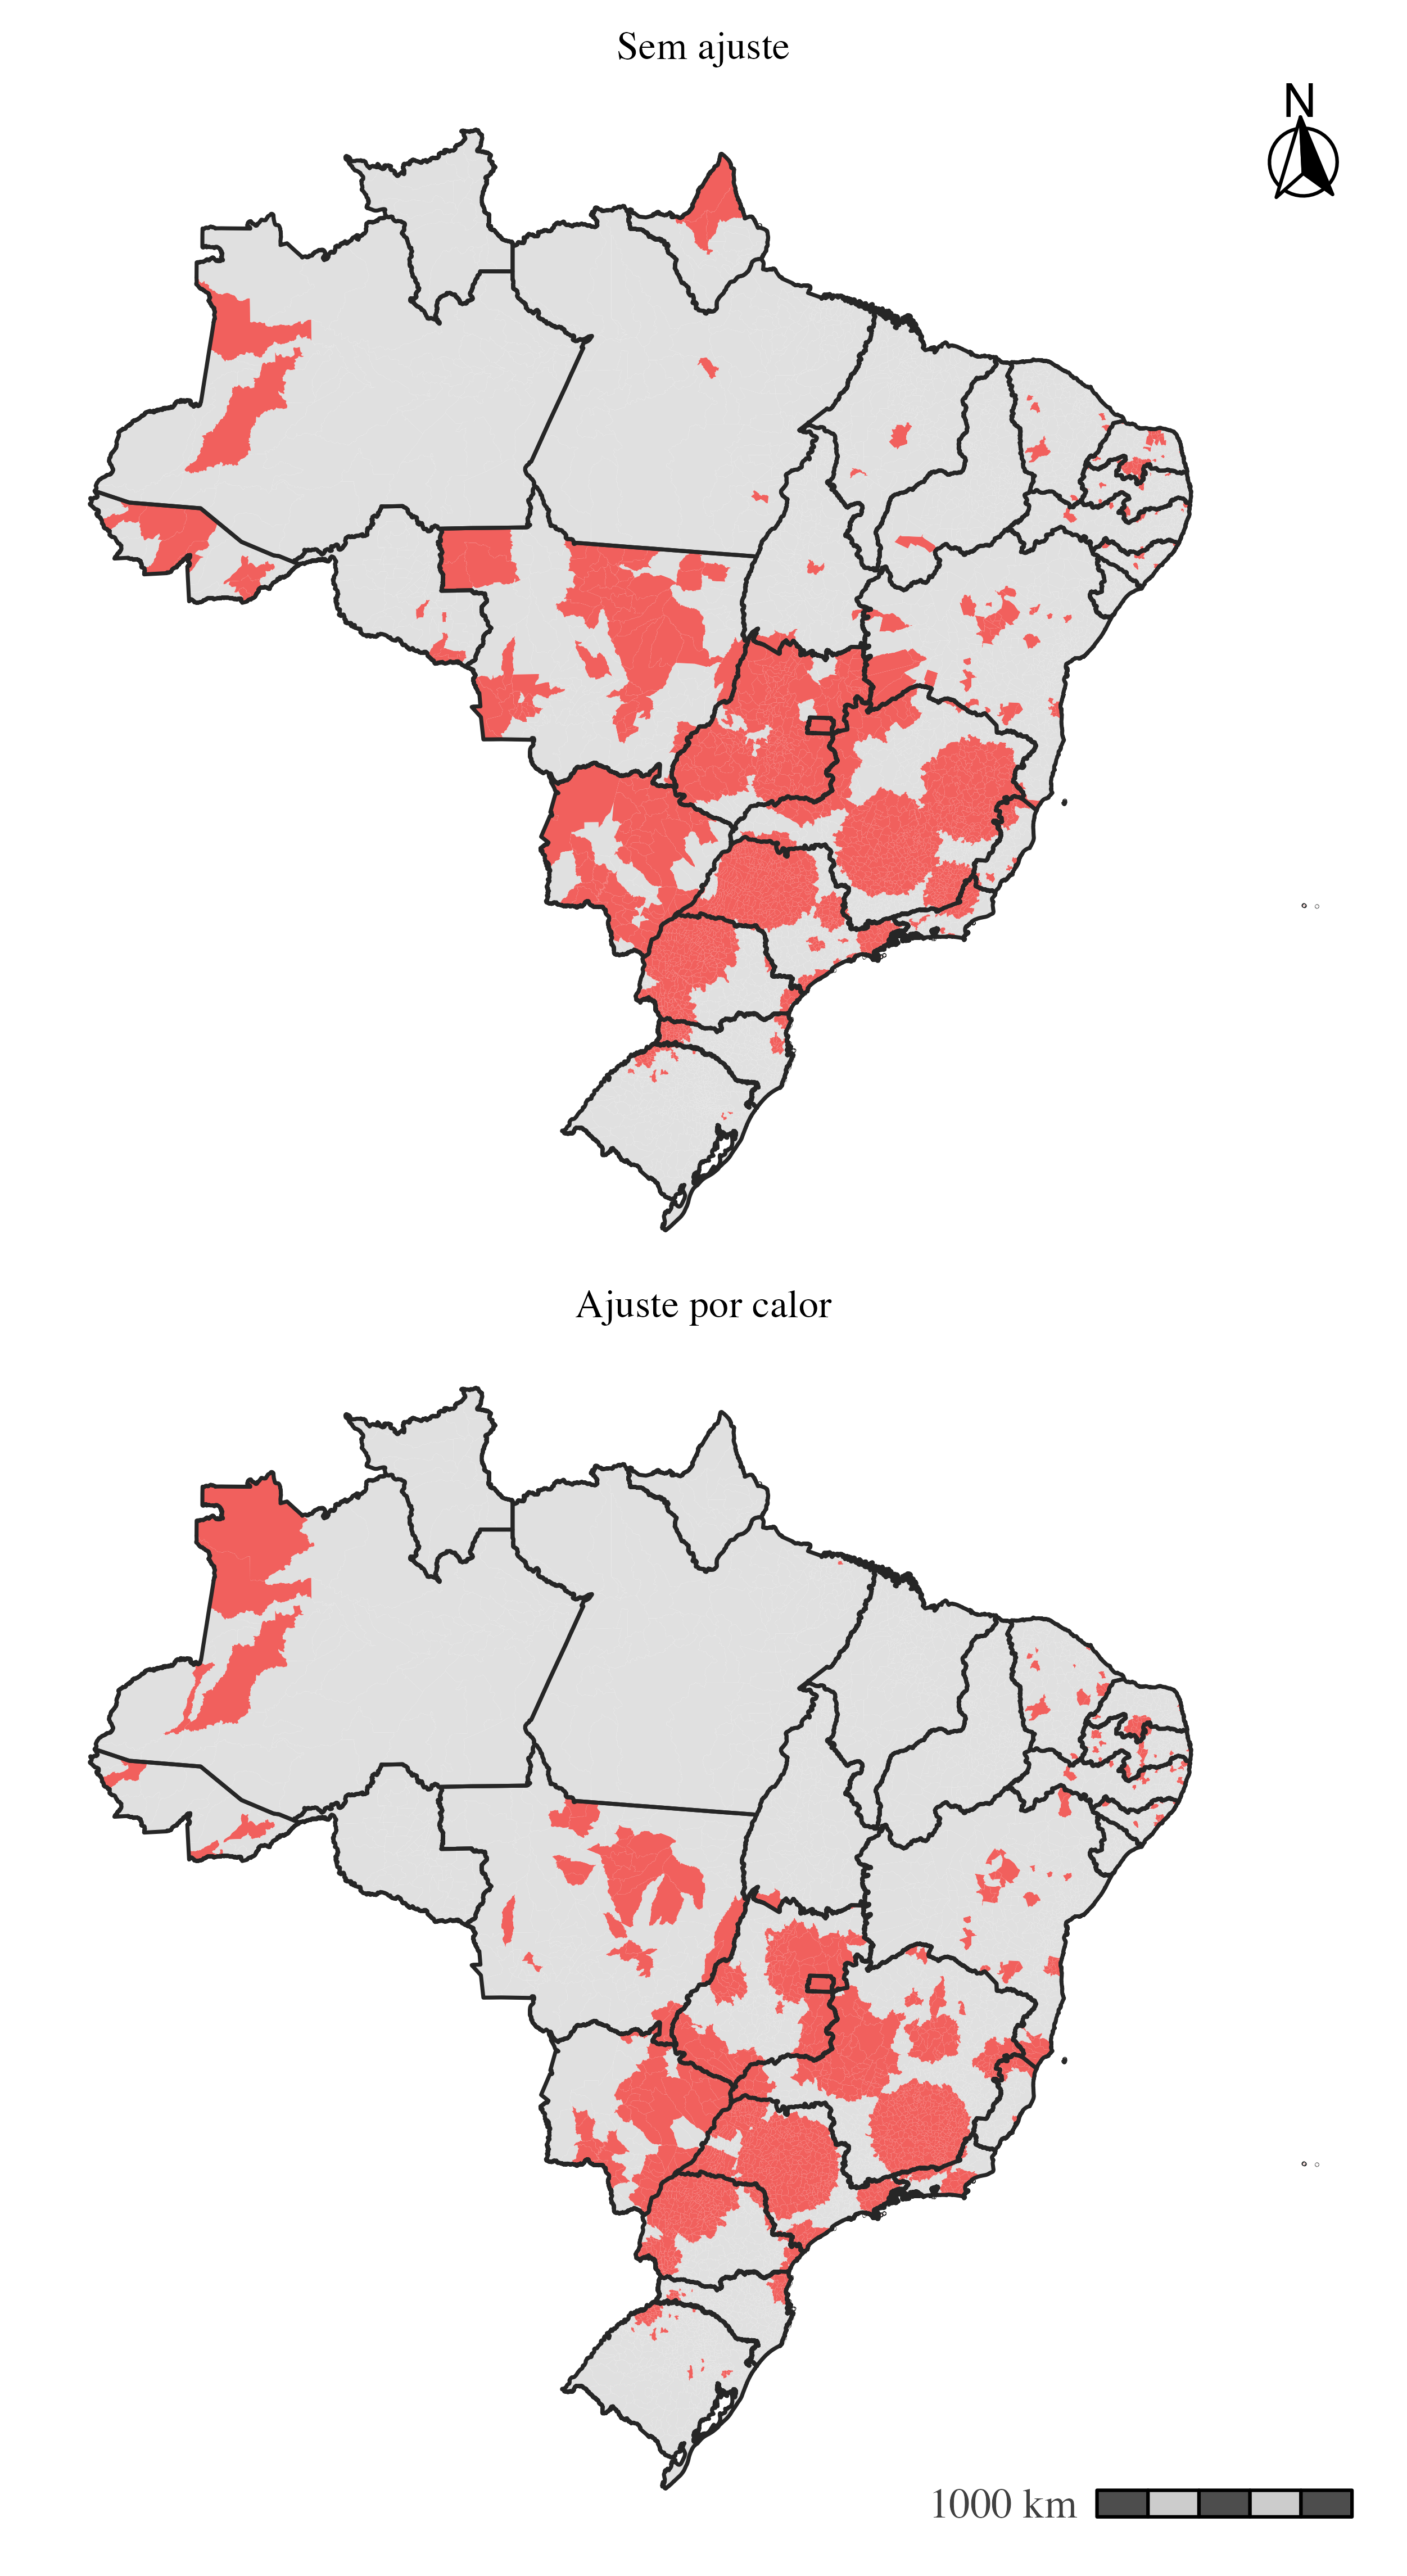
\includegraphics[width=0.66\textwidth]{fig_mapa_clusters_2x1_puro_calor.png}
    \caption{Zonas significativas de alto risco de dengue, Brasil, 2010--2025. (a) Sem ajuste. (b) Ajuste por calor. O modelo sem ajuste identificou 129 zonas sem sobreposição (nível de 5\%), com primário em Adolfo (SP), 319 municípios e risco relativo de 2,99, cobrindo 64,1\% dos casos do painel. O ajuste por calor identificou 128 zonas, com primário em Queluzito (MG), 362 municípios e risco relativo de 2,08, cobrindo 63,3\% dos casos. Fontes: SINAN e IBGE.}
    \label{fig:mapas_zonas}
    \vspace{0.3em}
    {\footnotesize\noindent\textit{Nota:} Em laranja, municípios em zonas com nível de 5\%; em cinza, municípios fora de zonas. Valores de casos, expectativa e risco relativo para 2010--2025.\par}
\end{figure}

\begin{figure}[H]
    \centering
    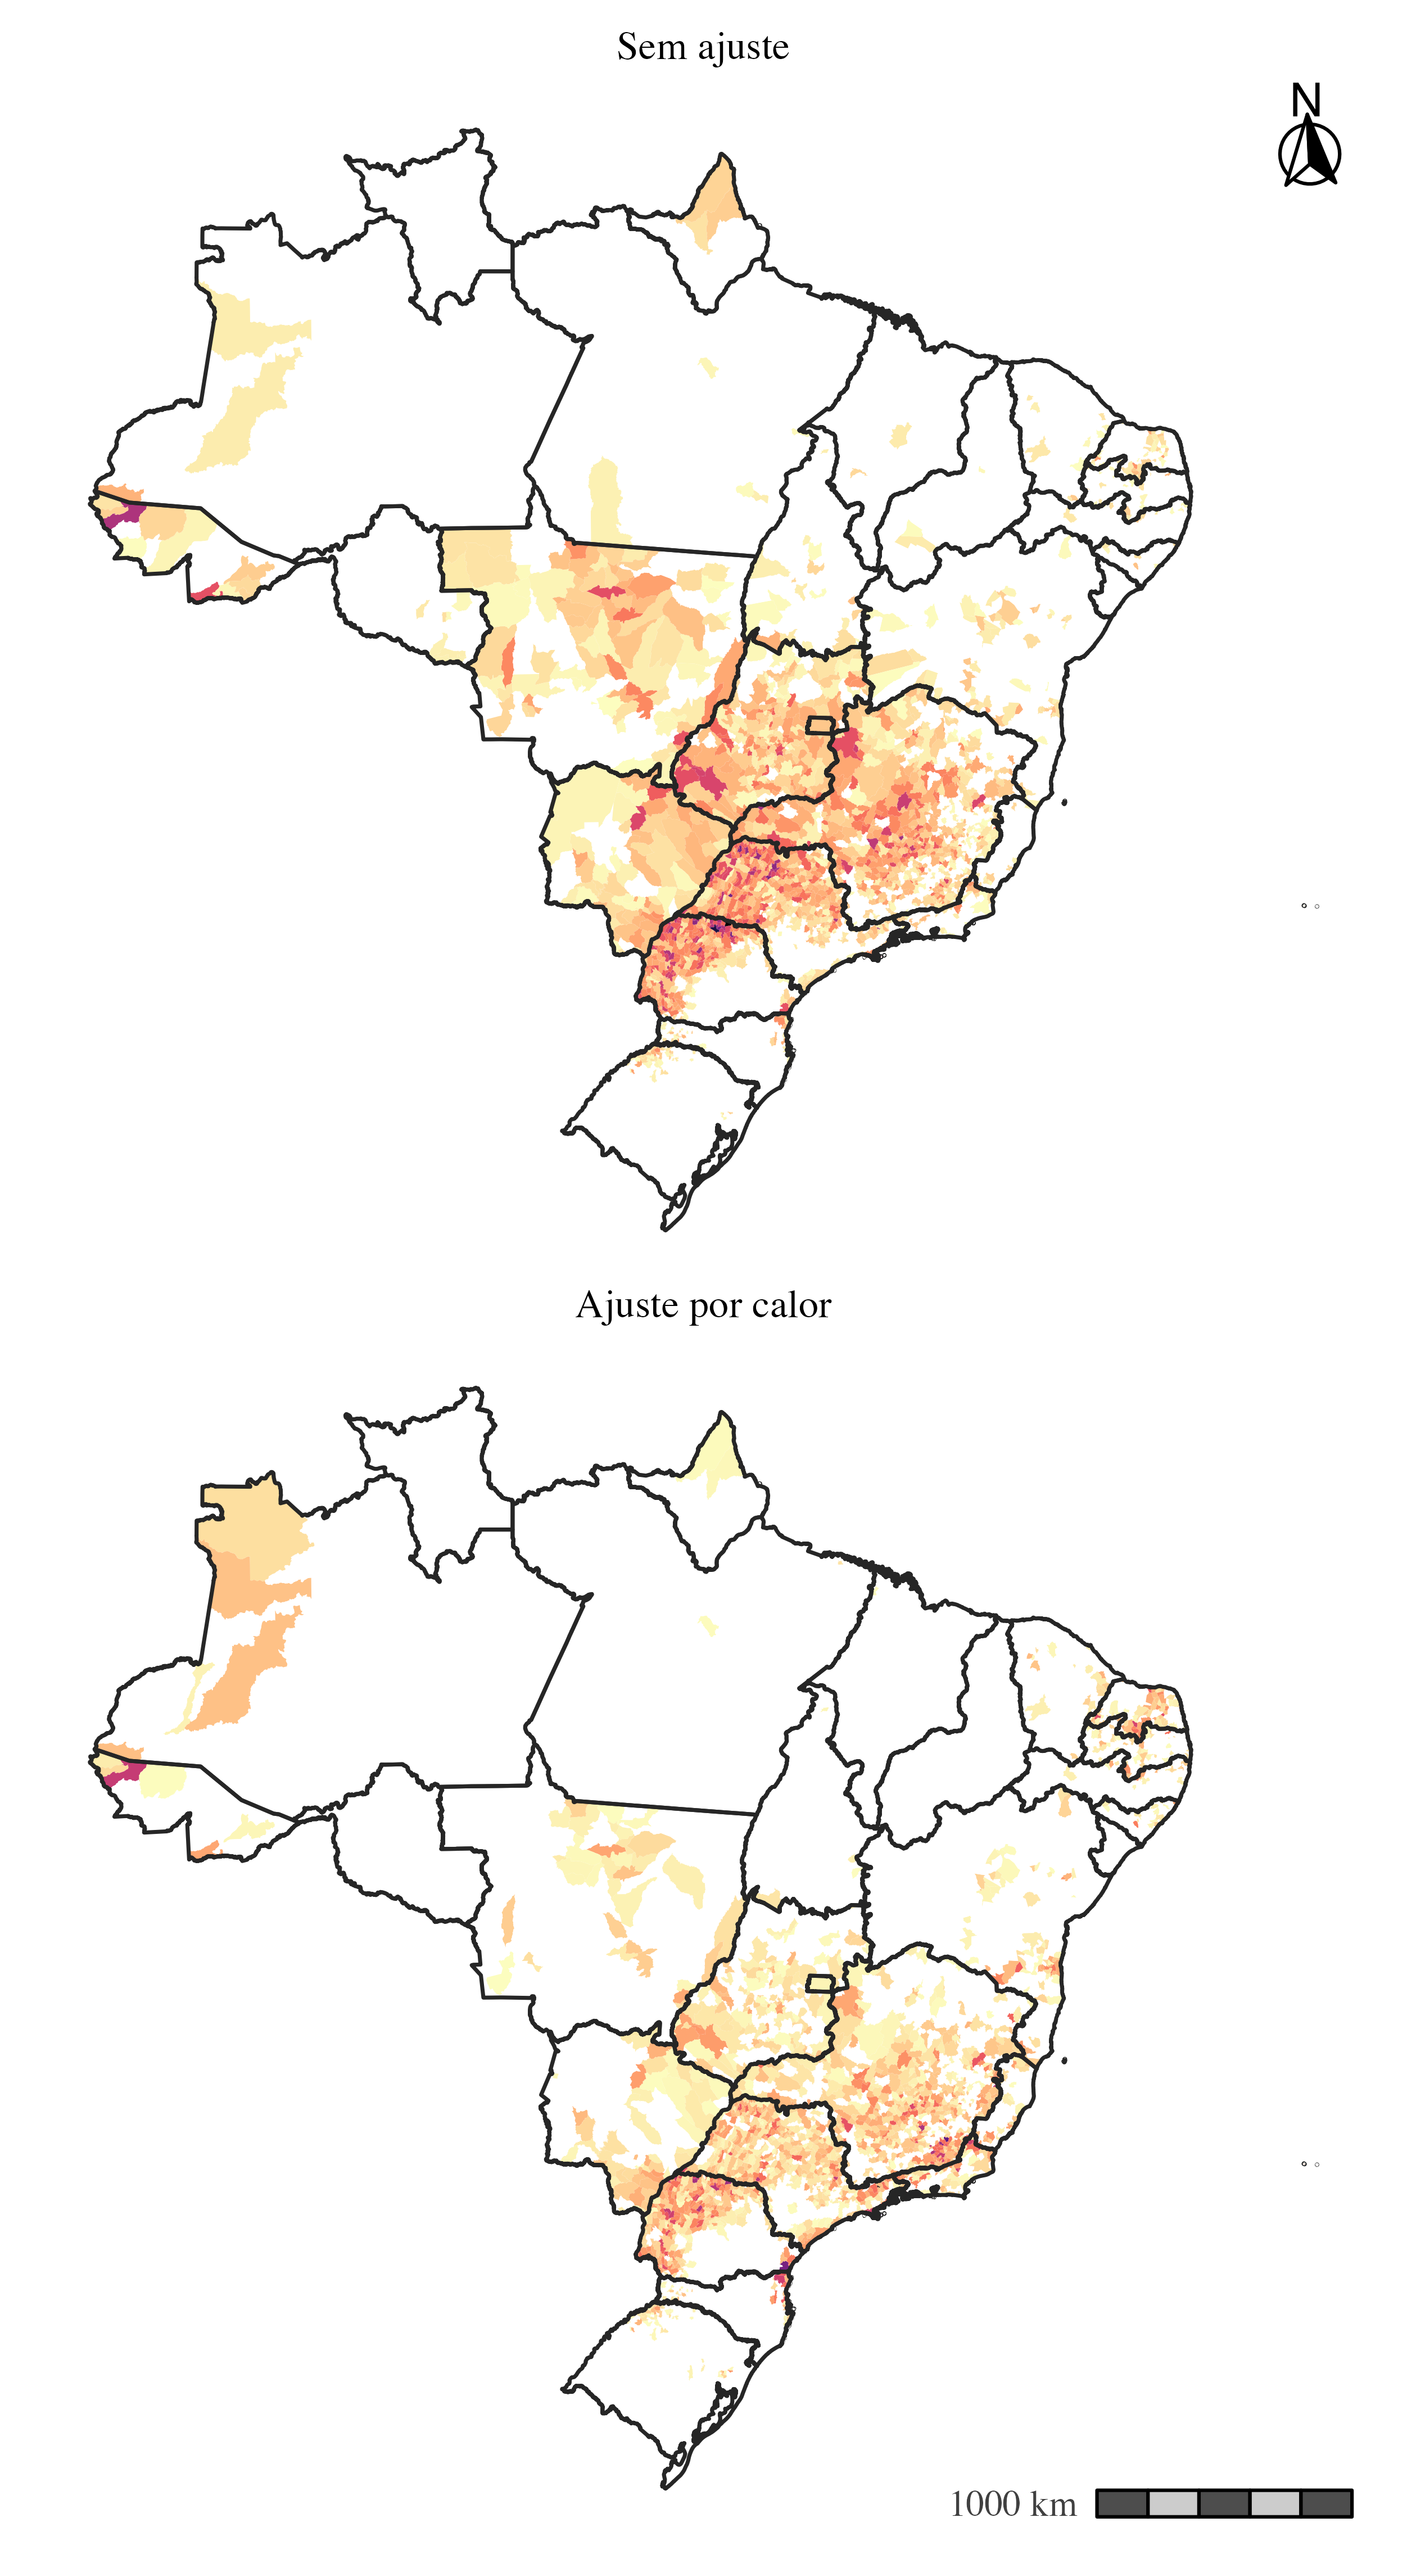
\includegraphics[width=0.66\textwidth]{fig_mapa_rr_2x1_puro_calor.png}
    \caption{Risco relativo municipal estimado pela varredura espacial sem ajuste (a) e sob ajuste por calor (b), Brasil, 2010--2025. Fontes: SINAN e IBGE.}
    \label{fig:mapas_rr}
    \vspace{0.3em}
    {\footnotesize\noindent\textit{Nota:} Tons mais escuros indicam risco relativo mais alto, na escala comum aos dois painéis, de 1,0 a 8,6; em branco, municípios com $RR \le 1{,}0$. O risco relativo é o reportado pelo programa sob a expectativa padronizada de cada modelo.\par}
\end{figure}

\subsection{Ajuste por calor}
\label{subsec:satscan_calor}

O ajuste por tercis de dias em onda de calor reteve 128 zonas, com cobertura de 1.679 municípios (30,2\%) e 13.989.139 casos (63,3\%) em 31,5\% da população. O primário deslocou-se para Queluzito (MG), com 362 municípios em raio de 199,5~km e $RR = 2{,}08$ (2.967.585 casos contra 1.533.663 esperados), seguido por Boracéia (SP), com 335 municípios ($RR = 1{,}86$), e por Goiânia (GO), janela compacta de 3 municípios em 18,8~km ($RR = 2{,}40$; 810.059 casos contra 344.386 esperados). A lista completa das 128 zonas consta do Apêndice~\ref{app:clusters_termica}.

As Figuras~\ref{fig:mapas_zonas} e \ref{fig:mapas_rr} comparam o modelo sem ajuste e o ajuste por calor. As Figuras~\ref{fig:prancha_clusters}, \ref{fig:prancha_clusters_sem2024} e \ref{fig:prancha_rr}, reunidas no Apêndice~\ref{app:pranchas}, apresentam, respectivamente, as zonas significativas das oito formulações no período completo, as zonas no cenário sem 2024 e os riscos relativos das seis formulações restantes. As Tabelas~\ref{tab:clusters_satscan_puro} e \ref{tab:clusters_satscan_termica}, nos Apêndices~\ref{app:clusters} e \ref{app:clusters_termica}, detalham as zonas municipais dos modelos sem ajuste e com ajuste por calor.

\subsection{Sensibilidade à exclusão de 2024}
\label{subsec:satscan_sens2024}

Para avaliar a sensibilidade ao ano epidêmico de 2024, as oito formulações foram reexecutadas sem os casos desse ano, com configuração idêntica (Figuras~\ref{fig:zonas_puro_2024} e \ref{fig:zonas_calor_2024}). A Tabela~\ref{tab:sensibilidade_satscan} apresenta o número de zonas, o polo primário e a sobreposição municipal entre os cenários. Sem 2024, o painel reúne 15.664.546 casos e o número de zonas significativas aumentou sem ajuste (de 129 para 169), sob calor (de 128 para 130), sob densidade urbana (de 136 para 168), sob proporção urbana (de 158 para 173) e sob o índice composto (de 184 para 196); sob esgoto, água e lixo, diminuiu ligeiramente. O polo primário sem ajuste deslocou-se de Adolfo (SP) para Ubarana (SP) e, sob calor, de Queluzito (MG) para Iacri (SP). A sobreposição municipal entre os cenários variou de 51\% (calor) a 63\% (esgoto). O WMAPE foi maior no cenário sem 2024 em todas as formulações (por exemplo, 81,0\% sem ajuste e 71,0\% sob calor), mas a ordenação relativa no topo foi preservada: calor e água permaneceram os menores valores nos dois cenários.

\begin{table}[!h]
\centering
\caption{\label{tab:sensibilidade_satscan}Sensibilidade à exclusão de 2024 na varredura espacial: número de zonas, polo primário e sobreposição municipal entre os cenários (2010--2025 e sem 2024), Brasil.}
\centering
\resizebox{\ifdim\width>\linewidth\linewidth\else\width\fi}{!}{
\fontsize{9}{11}\selectfont
\begin{tabular}[t]{lccllc}
\toprule
\multicolumn{1}{c}{ } & \multicolumn{2}{c}{Zonas (n)} & \multicolumn{2}{c}{Polo primário} & \multicolumn{1}{c}{Sobreposição entre cenários} \\
\cmidrule(l{3pt}r{3pt}){2-3} \cmidrule(l{3pt}r{3pt}){4-5} \cmidrule(l{3pt}r{3pt}){6-6}
Ajuste & Com 2024 & Sem 2024 & Com 2024 & Sem 2024 & Jaccard\\
\midrule
Sem ajuste & 129 & 169 & Adolfo (SP) & Ubarana (SP) & 61\%\\
Calor & 128 & 130 & Queluzito (MG) & Iacri (SP) & 51\%\\
Esgoto adequado & 178 & 174 & Iacri (SP) & Iacri (SP) & 63\%\\
Densidade urbana & 136 & 168 & Araújos (MG) & Ubarana (SP) & 55\%\\
Proporção urbana & 158 & 173 & Iacri (SP) & Ubarana (SP) & 58\%\\
\addlinespace
Água por rede & 193 & 188 & Iacri (SP) & Ubarana (SP) & 60\%\\
Coleta de lixo & 195 & 186 & Iacri (SP) & Ubarana (SP) & 60\%\\
Índice composto & 184 & 196 & Araújos (MG) & Ubarana (SP) & 61\%\\
\bottomrule
\end{tabular}}
\end{table}


\clearpage
\begin{figure}[H]
    \centering
    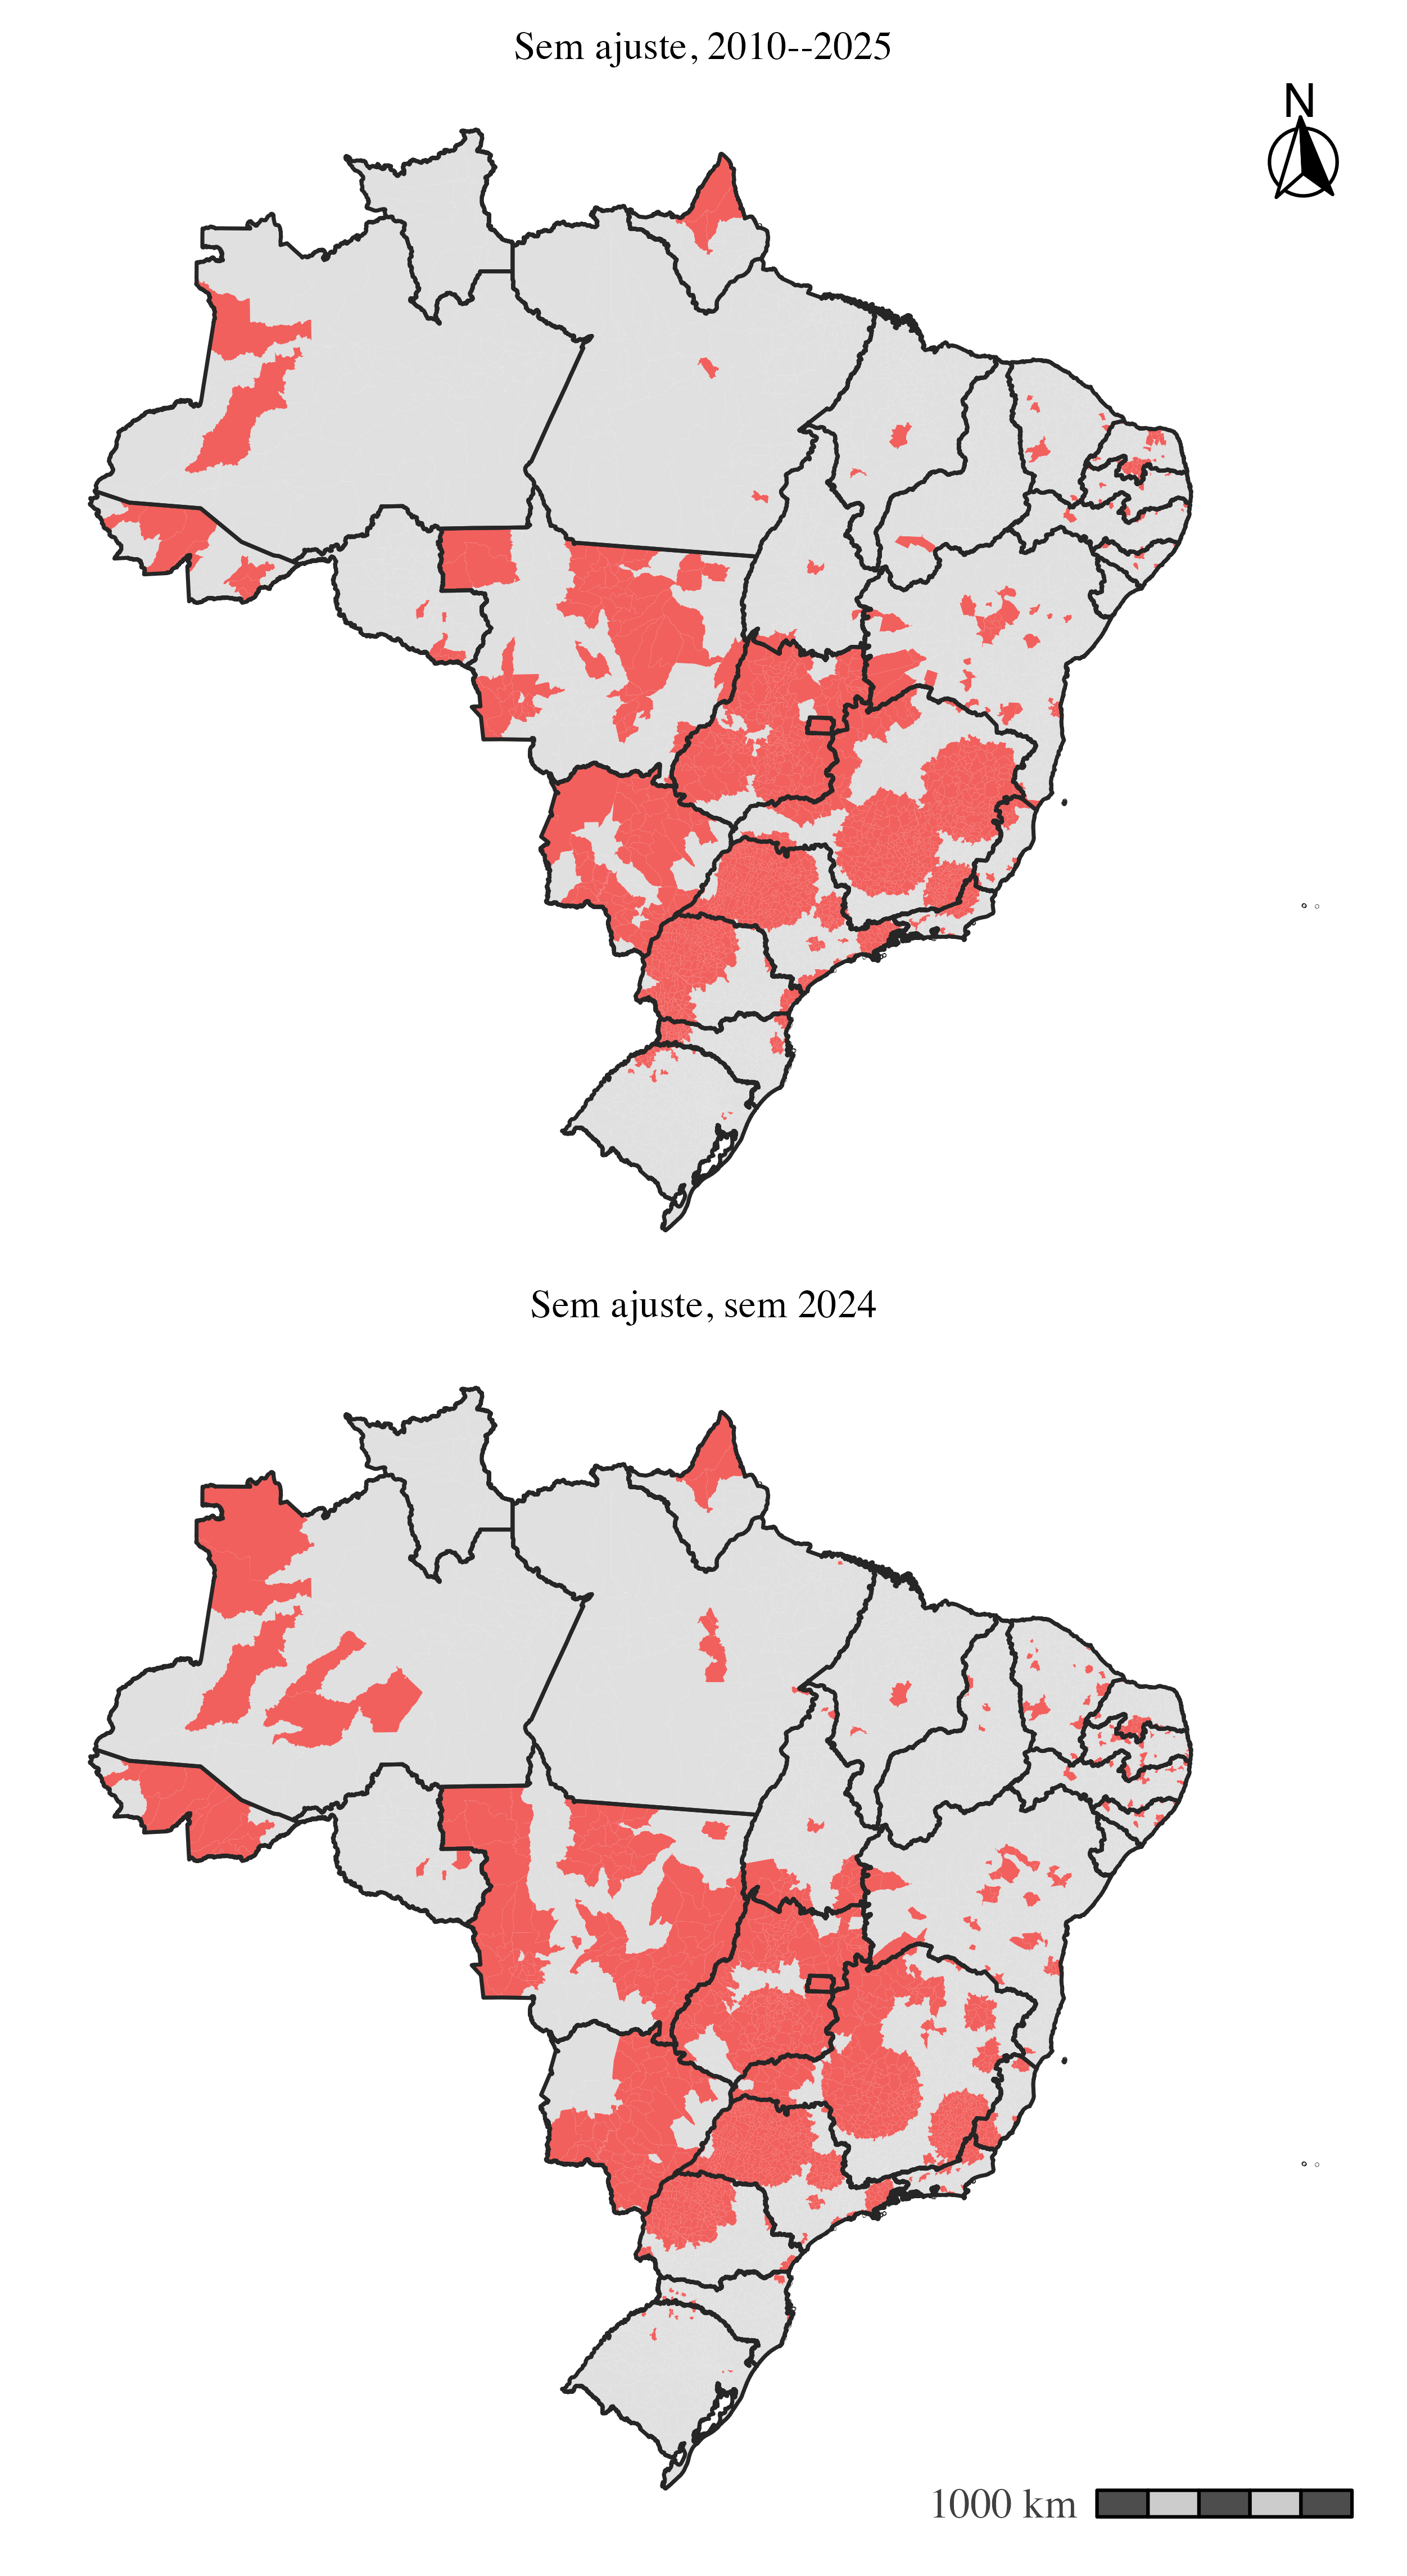
\includegraphics[width=0.66\textwidth]{fig_mapa_clusters_2x1_puro_com_sem2024.png}
    \caption{Zonas de alta incidência no modelo sem ajuste com os casos de 2024 (a) e sem os casos de 2024 (b), Brasil. Fontes: SINAN e IBGE.}
    \label{fig:zonas_puro_2024}
    \vspace{0.3em}
    {\footnotesize\noindent\textit{Nota:} Em laranja, municípios em zonas com nível de 5\%; em cinza, municípios fora de zonas. Os dois painéis usam a mesma configuração espacial e o mesmo limite de 16\% da população e 200~km.\par}
\end{figure}

\begin{figure}[H]
    \centering
    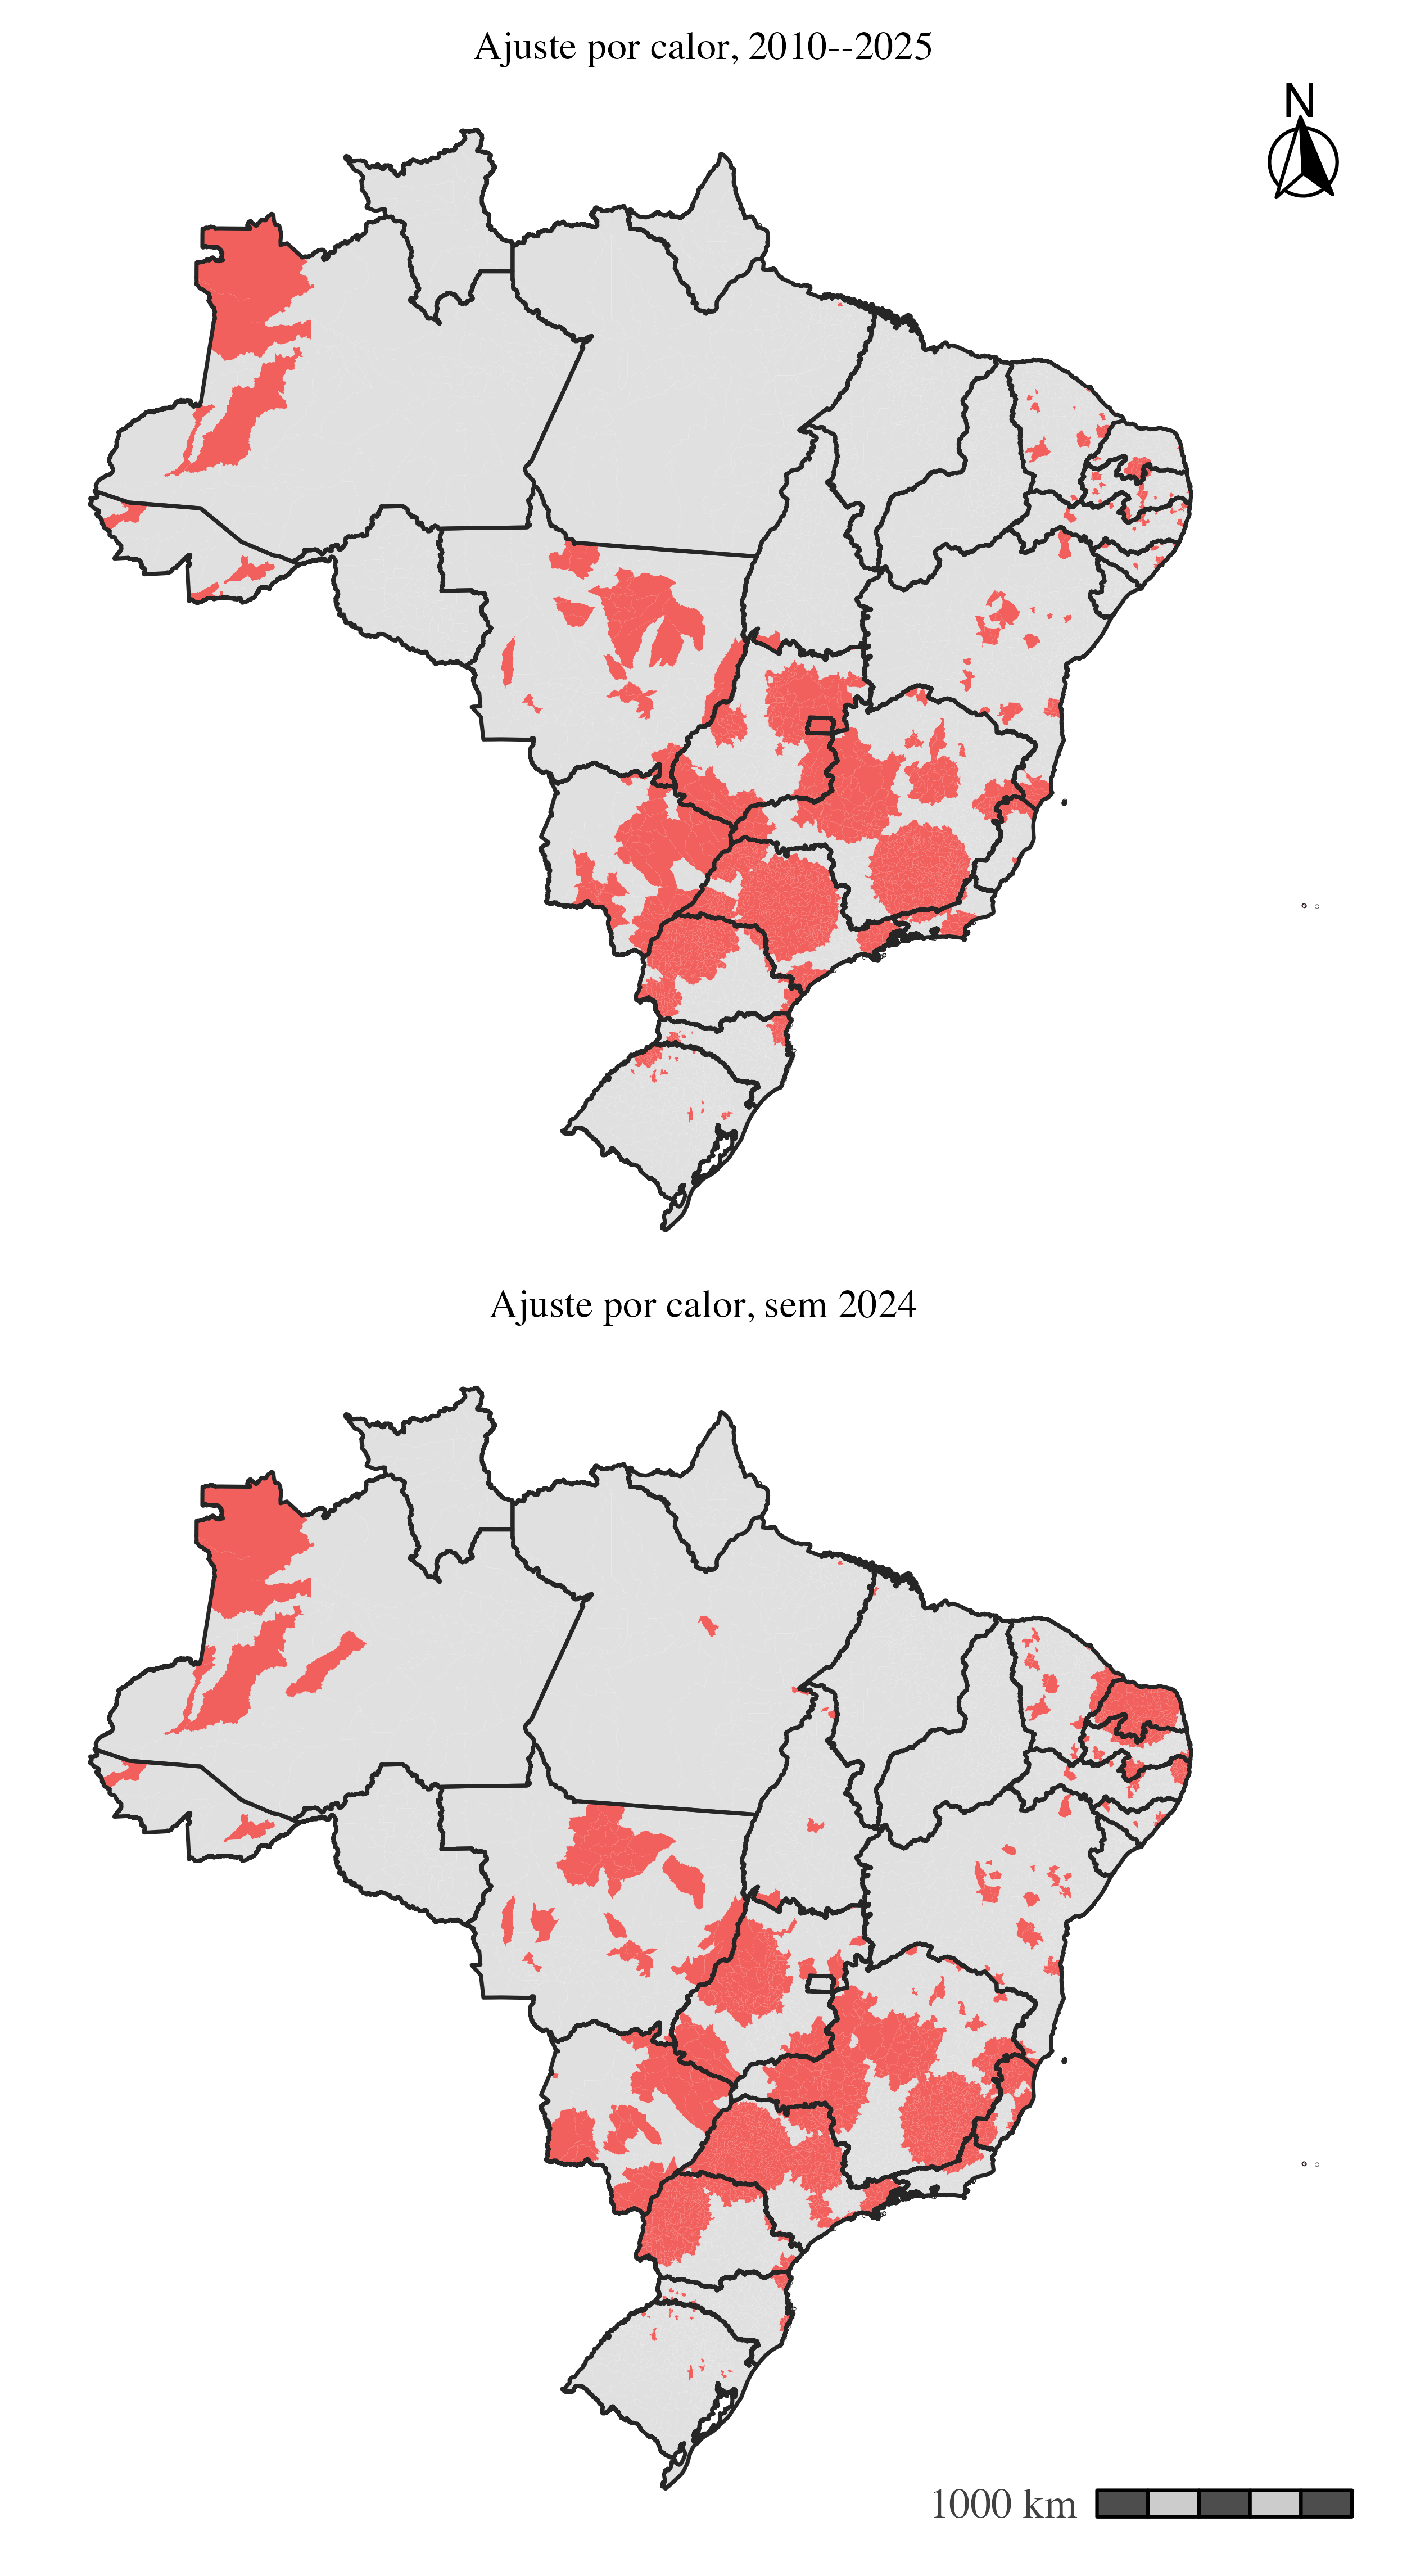
\includegraphics[width=0.66\textwidth]{fig_mapa_clusters_2x1_calor_com_sem2024.png}
    \caption{Zonas de alta incidência sob ajuste por calor com os casos de 2024 (a) e sem os casos de 2024 (b), Brasil. Fontes: SINAN e IBGE.}
    \label{fig:zonas_calor_2024}
    \vspace{0.3em}
    {\footnotesize\noindent\textit{Nota:} Mesma codificação de cor e mesma configuração espacial nos dois painéis; a comparação isola o efeito do período, mantida a padronização pelos tercis de calor.\par}
\end{figure}

